\documentclass[]{article}
\usepackage{lmodern}
\usepackage{amssymb,amsmath}
\usepackage{ifxetex,ifluatex}
\usepackage{fixltx2e} % provides \textsubscript
\ifnum 0\ifxetex 1\fi\ifluatex 1\fi=0 % if pdftex
  \usepackage[T1]{fontenc}
  \usepackage[utf8]{inputenc}
\else % if luatex or xelatex
  \ifxetex
    \usepackage{mathspec}
  \else
    \usepackage{fontspec}
  \fi
  \defaultfontfeatures{Ligatures=TeX,Scale=MatchLowercase}
\fi
% use upquote if available, for straight quotes in verbatim environments
\IfFileExists{upquote.sty}{\usepackage{upquote}}{}
% use microtype if available
\IfFileExists{microtype.sty}{%
\usepackage{microtype}
\UseMicrotypeSet[protrusion]{basicmath} % disable protrusion for tt fonts
}{}
\usepackage[margin=1in]{geometry}
\usepackage{hyperref}
\hypersetup{unicode=true,
            pdftitle={Laborator 5},
            pdfborder={0 0 0},
            breaklinks=true}
\urlstyle{same}  % don't use monospace font for urls
\usepackage{natbib}
\bibliographystyle{plainnat}
\usepackage{color}
\usepackage{fancyvrb}
\newcommand{\VerbBar}{|}
\newcommand{\VERB}{\Verb[commandchars=\\\{\}]}
\DefineVerbatimEnvironment{Highlighting}{Verbatim}{commandchars=\\\{\}}
% Add ',fontsize=\small' for more characters per line
\usepackage{framed}
\definecolor{shadecolor}{RGB}{248,248,248}
\newenvironment{Shaded}{\begin{snugshade}}{\end{snugshade}}
\newcommand{\KeywordTok}[1]{\textcolor[rgb]{0.13,0.29,0.53}{\textbf{#1}}}
\newcommand{\DataTypeTok}[1]{\textcolor[rgb]{0.13,0.29,0.53}{#1}}
\newcommand{\DecValTok}[1]{\textcolor[rgb]{0.00,0.00,0.81}{#1}}
\newcommand{\BaseNTok}[1]{\textcolor[rgb]{0.00,0.00,0.81}{#1}}
\newcommand{\FloatTok}[1]{\textcolor[rgb]{0.00,0.00,0.81}{#1}}
\newcommand{\ConstantTok}[1]{\textcolor[rgb]{0.00,0.00,0.00}{#1}}
\newcommand{\CharTok}[1]{\textcolor[rgb]{0.31,0.60,0.02}{#1}}
\newcommand{\SpecialCharTok}[1]{\textcolor[rgb]{0.00,0.00,0.00}{#1}}
\newcommand{\StringTok}[1]{\textcolor[rgb]{0.31,0.60,0.02}{#1}}
\newcommand{\VerbatimStringTok}[1]{\textcolor[rgb]{0.31,0.60,0.02}{#1}}
\newcommand{\SpecialStringTok}[1]{\textcolor[rgb]{0.31,0.60,0.02}{#1}}
\newcommand{\ImportTok}[1]{#1}
\newcommand{\CommentTok}[1]{\textcolor[rgb]{0.56,0.35,0.01}{\textit{#1}}}
\newcommand{\DocumentationTok}[1]{\textcolor[rgb]{0.56,0.35,0.01}{\textbf{\textit{#1}}}}
\newcommand{\AnnotationTok}[1]{\textcolor[rgb]{0.56,0.35,0.01}{\textbf{\textit{#1}}}}
\newcommand{\CommentVarTok}[1]{\textcolor[rgb]{0.56,0.35,0.01}{\textbf{\textit{#1}}}}
\newcommand{\OtherTok}[1]{\textcolor[rgb]{0.56,0.35,0.01}{#1}}
\newcommand{\FunctionTok}[1]{\textcolor[rgb]{0.00,0.00,0.00}{#1}}
\newcommand{\VariableTok}[1]{\textcolor[rgb]{0.00,0.00,0.00}{#1}}
\newcommand{\ControlFlowTok}[1]{\textcolor[rgb]{0.13,0.29,0.53}{\textbf{#1}}}
\newcommand{\OperatorTok}[1]{\textcolor[rgb]{0.81,0.36,0.00}{\textbf{#1}}}
\newcommand{\BuiltInTok}[1]{#1}
\newcommand{\ExtensionTok}[1]{#1}
\newcommand{\PreprocessorTok}[1]{\textcolor[rgb]{0.56,0.35,0.01}{\textit{#1}}}
\newcommand{\AttributeTok}[1]{\textcolor[rgb]{0.77,0.63,0.00}{#1}}
\newcommand{\RegionMarkerTok}[1]{#1}
\newcommand{\InformationTok}[1]{\textcolor[rgb]{0.56,0.35,0.01}{\textbf{\textit{#1}}}}
\newcommand{\WarningTok}[1]{\textcolor[rgb]{0.56,0.35,0.01}{\textbf{\textit{#1}}}}
\newcommand{\AlertTok}[1]{\textcolor[rgb]{0.94,0.16,0.16}{#1}}
\newcommand{\ErrorTok}[1]{\textcolor[rgb]{0.64,0.00,0.00}{\textbf{#1}}}
\newcommand{\NormalTok}[1]{#1}
\usepackage{longtable,booktabs}
\usepackage{graphicx,grffile}
\makeatletter
\def\maxwidth{\ifdim\Gin@nat@width>\linewidth\linewidth\else\Gin@nat@width\fi}
\def\maxheight{\ifdim\Gin@nat@height>\textheight\textheight\else\Gin@nat@height\fi}
\makeatother
% Scale images if necessary, so that they will not overflow the page
% margins by default, and it is still possible to overwrite the defaults
% using explicit options in \includegraphics[width, height, ...]{}
\setkeys{Gin}{width=\maxwidth,height=\maxheight,keepaspectratio}
\IfFileExists{parskip.sty}{%
\usepackage{parskip}
}{% else
\setlength{\parindent}{0pt}
\setlength{\parskip}{6pt plus 2pt minus 1pt}
}
\setlength{\emergencystretch}{3em}  % prevent overfull lines
\providecommand{\tightlist}{%
  \setlength{\itemsep}{0pt}\setlength{\parskip}{0pt}}
\setcounter{secnumdepth}{5}
% Redefines (sub)paragraphs to behave more like sections
\ifx\paragraph\undefined\else
\let\oldparagraph\paragraph
\renewcommand{\paragraph}[1]{\oldparagraph{#1}\mbox{}}
\fi
\ifx\subparagraph\undefined\else
\let\oldsubparagraph\subparagraph
\renewcommand{\subparagraph}[1]{\oldsubparagraph{#1}\mbox{}}
\fi

%%% Use protect on footnotes to avoid problems with footnotes in titles
\let\rmarkdownfootnote\footnote%
\def\footnote{\protect\rmarkdownfootnote}

%%% Change title format to be more compact
\usepackage{titling}

% Create subtitle command for use in maketitle
\newcommand{\subtitle}[1]{
  \posttitle{
    \begin{center}\large#1\end{center}
    }
}

\setlength{\droptitle}{-2em}
  \title{Laborator 5}
  \pretitle{\vspace{\droptitle}\centering\huge}
  \posttitle{\par}
\subtitle{Elemente de regresie liniară simplă}
  \author{}
  \preauthor{}\postauthor{}
  \date{}
  \predate{}\postdate{}

\usepackage{booktabs}
\usepackage{longtable}
\usepackage{framed,color}
\definecolor{shadecolor}{RGB}{248, 248, 248}
%\definecolor{shadecolor1}{RGB}{216,225,235}
%\definecolor{framecolor}{RGB}{108,123,13}

%\definecolor{shadecolor}{RGB}{226, 255, 241}
\definecolor{shadecolor1}{RGB}{217,225,199}
\definecolor{framecolor}{RGB}{60,179,113}

\ifxetex
  \usepackage{letltxmacro}
  \setlength{\XeTeXLinkMargin}{1pt}
  \LetLtxMacro\SavedIncludeGraphics\includegraphics
  \def\includegraphics#1#{% #1 catches optional stuff (star/opt. arg.)
    \IncludeGraphicsAux{#1}%
  }%
  \newcommand*{\IncludeGraphicsAux}[2]{%
    \XeTeXLinkBox{%
      \SavedIncludeGraphics#1{#2}%
    }%
  }%
\fi

\newenvironment{frshaded*}{%
  \def\FrameCommand{\fboxrule=\FrameRule\fboxsep=\FrameSep \fcolorbox{framecolor}{shadecolor1}}%
  \MakeFramed {\advance\hsize-\width \FrameRestore}}%
{\endMakeFramed}

\newenvironment{rmdblock}[1]
  {\begin{frshaded*}
  \begin{itemize}
  \renewcommand{\labelitemi}{
    \raisebox{-.7\height}[0pt][0pt]{
      {\setkeys{Gin}{width=2em,keepaspectratio}\includegraphics{images/icons/#1}}
    }
  }
  \item
  }
  {
  \end{itemize}
  \end{frshaded*}
  }

\newenvironment{rmdcaution}
  {\begin{rmdblock}{caution}}
  {\end{rmdblock}}
% \newenvironment{rmdinsight}
%   {\begin{rmdblock}{insight}}
%   {\end{rmdblock}}
\newenvironment{rmdexercise}
  {\begin{rmdblock}{exercise}}
  {\end{rmdblock}}
\newenvironment{rmdtip}
  {\begin{rmdblock}{tip}}
  {\end{rmdblock}}


%%%%%%%%%%%%%%%%%%%%%%%%%%%%%%%%%%%%%%%%%%%%%%%%%%%%%%%%%%%%%%%%%%%%%%%%%%%%%%%%%%%%%%%%%%%%%%%%%%%%%%%%%%%%%%%%%%%%%
%%%%%%%%%%% For insight block %%%%%%%%%%%%%%%%%%%%%%%%%%
\definecolor{shadecolor_insight}{RGB}{223,240,216}
\definecolor{framecolor_insight}{RGB}{136,193,137}

%\definecolor{shadecolor_insight}{RGB}{217,225,199}
%\definecolor{framecolor_insight}{RGB}{60,179,113}

\newenvironment{frshaded_insight*}{%
  \def\FrameCommand{\fboxrule=\FrameRule\fboxsep=\FrameSep \fcolorbox{framecolor_insight}{shadecolor_insight}}%
  \MakeFramed {\advance\hsize-\width \FrameRestore}}%
{\endMakeFramed}

\newenvironment{rmdblock_insight}[1]
  {\begin{frshaded_insight*}
  \begin{itemize}
  \renewcommand{\labelitemi}{
    \raisebox{-.7\height}[0pt][0pt]{
      {\setkeys{Gin}{width=2em,keepaspectratio}\includegraphics{images/icons/#1}}
    }
  }
  \item
  }
  {
  \end{itemize}
  \end{frshaded_insight*}
  }

\newenvironment{rmdinsight}
  {\begin{rmdblock_insight}{insight}}
  {\end{rmdblock_insight}}

%%%%%%%%%%%%%%%%%%%%%%%%%%%%%%%%%%%%%%%%%%%%%%%%%%%%%%%%%%%%%%%%%%%%%%%%%%%%%%%%%%%%%%%%%%%%%%%%%%%%%%%%%%%%%%%%%%%%%
\usepackage{subfigure}
\usepackage{booktabs}
\usepackage{slashbox}
\usepackage{color}
%%%%%%%%%%%%%%%%%%%%%%%%%%%%%%%%%%%%%%%%%
\definecolor{linkcol}{rgb}{0,0,0.4}
\definecolor{citecol}{rgb}{0.5,0,0}

% Change this to change the informations included in the pdf file
% \usepackage[pagebackref]{hyperref}
% \usepackage[verbose]{backref}
\usepackage[hyperpageref]{backref}
% \backrefsetup{verbose=false}
% \PassOptionsToPackage{pagebackref}{hyperref}
% See hyperref documentation for information on those parameters

\hypersetup
{
bookmarksopen=true,
pdftitle="Curs Instrumente Statistice pentru Finante",
pdfauthor="Alexandru Amarioarei",
pdfsubject="Laboratoare Instrumente Statistice pentru Finante", %subject of the document
pdfmenubar=true, %menubar shown
pdfhighlight=/O, %effect of clicking on a link
colorlinks=true, %couleurs sur les liens hypertextes
pdfpagemode=None, %aucun mode de page
pdfpagelayout=SinglePage, %ouverture en simple page
pdffitwindow=true, %pages ouvertes entierement dans toute la fenetre
linkcolor=linkcol, %couleur des liens hypertextes internes
citecolor=citecol, %couleur des liens pour les citations
urlcolor=linkcol %couleur des liens pour les url
}


% set the back references
\renewcommand*{\backref}[1]{}
\renewcommand*{\backreftwosep}{ și~} % inserted between entries 
                              % in a list of two entries, 
                              % default is " and~".
\renewcommand*{\backreflastsep}{ și~} % inserted between the last 
                               % two entries of a list with more
                               % than two entries, default is ", and~".
\renewcommand*{\backrefalt}[4]{%
    \ifcase #1 (Necitat.)%
    \or        (Citat la pagina~#2.)%
    \else      (Citat la paginile~#2.)%
    \fi}

%%%%%%%%%%%%%%%%%%%%%%%%%%%%%%%%%%%%%%%%%%%%%%%%%%%%%%%%%%%%%%%%%%%%%%%%%%%%%%%%%%%%%%%%%%%%%%%%%%%%%%%%%%%%%%%%%%%%%
%CITEVA DEFINITII
\def\om{\omega}
\def\Om{\Omega}
\def\et{\eta}
\def\td{\tilde{\delta}}
\def\m{{\mu}}
\def\n{{\nu}}
\def\k{{\kappa}}
\def\l{{\lambda}}
\def\L{{\Lambda}}
\def\g{{\gamma}}
\def\a{{\alpha}}
\def\e{{\varepsilon}}
\def\b{{\beta}}
\def\G{{\Gamma}}
\def\d{{\delta}}
\def\D{{\Delta}}
\def\t{{\theta}}
\def\s{{\sigma}}
\def\S{{\Sigma}}
\def\z{{\zeta}}
\def\qed{\hfill\Box}
\def\ds{\displaystyle}
\def\mc{\mathcal}
%%%%%%%%%%%%%%%%%%%%%%%%%%%%%%%%%%%%%%%%%%%%%%%%%%%%%%%%%%%%%%%%%%%%%%%%%%%%%%%%%%%%%%%%%%%%%%%%%%%%%%%%%%%%%%%%%%%%%%
\def\1{{\mathbf 1}}
\def\CC{{\mathbb C}}
\def\VV{{\mathbb V}}
\def\RR{{\mathbb R}}
\def\QQ{{\mathbb Q}}
\def\ZZ{{\mathbb Z}}
\def\PP{{\mathbb P}}
\def\EE{{\mathbb E}}
\def\NN{{\mathbb N}}
\def\FF{{\mathbb F}}
%\def\SS{{\mathbb S}}
\def\MA{{\mathcal A}}
\def\MO{{\mathcal O}}
\def\MF{{\mathcal F}}
\def\ME{{\mathcal E}}
\def\MR{{\mathcal R}}
\def\MB{{\mathcal B}}
\def\MM{{\mathcal M}}
\def\MN{{\mathcal N}}
\def\MU{{\mathcal U}}
\def\MP{{\mathcal P}}
\def\MS{{\mathcal S}}
\def\MBS{{\mathbf S}}
\def\MX{{\bm{ \mathscr X}}}

% independent sign
\newcommand\independent{\protect\mathpalette{\protect\independenT}{\perp}}
\def\independenT#1#2{\mathrel{\rlap{$#1#2$}\mkern2mu{#1#2}}}

\renewcommand\tablename{Tab.}
\renewcommand{\figurename}{Fig.}
\renewcommand\refname{Referințe}

%%%%%%%%%%%%%%%%%%%%%%%%%%%%%%%%%%%%%%%%%%%%%%%%%%%%%%%%%%%%%%%%%%%%%%%%%%%%%%%%%%%%%%%%%%%%%%%%%%%%%%%%%%%%%%%%%%%%%
%Header and Footer
\usepackage{fancyhdr}

\pagestyle{fancy}
\fancyhf{}
\rhead{Universitatea din Bucure\c sti\\ Facultatea de Matematic\u a \c si Informatic\u a}
\lhead{\textit{Curs}: Instrumente Statistice pentru Finan\c te\\ \textit{Instructor}: A. Am\u arioarei}
\rfoot{Pagina \thepage}
\lfoot{Grupa: 403}
%%%%%%%%%%%%%%%%%%%%%%%%%%%%%%%%%%%%%%%
\usepackage{booktabs}
\usepackage{longtable}
\usepackage{array}
\usepackage{multirow}
\usepackage[table]{xcolor}
\usepackage{wrapfig}
\usepackage{float}
\usepackage{colortbl}
\usepackage{pdflscape}
\usepackage{tabu}
\usepackage{threeparttable}
\usepackage{threeparttablex}
\usepackage[normalem]{ulem}
\usepackage{makecell}

\begin{document}
\maketitle

%%%%%%%%%%%%%%%%%%%%%%%%
\thispagestyle{fancy}

Obiectivul acestui laborator este de a prezenta câteva exemple legate de
problema de regresie liniară simplă.

\section{Introducere}\label{introducere}

Regresia liniară simplă (sau \emph{modelul liniar simplu}) este un
instrument statistic utilizat pentru a descrie relația dintre două
variabile aleatoare, \(X\) (variabilă \emph{cauză}, \emph{predictor} sau
\emph{covariabilă}) și \(Y\) (variabilă \emph{răspuns} sau \emph{efect})
și este definit prin

\[
\mathbb{E}[Y|X=x]=\beta_0+\beta_1x 
\]

sau altfel spus

\[
Y = \beta_0 + \beta_1 X + \varepsilon.
\]

În relațiile de mai sus, \(\beta_0\) și \(\beta_1\) sunt cunoscute ca
ordonata la origine (\emph{intercept}) și respectiv panta (\emph{slope})
dreptei de regresie.

Ipotezele modelului sunt:

\begin{enumerate}
\def\labelenumi{\roman{enumi}.}
\item
  \textbf{Linearitatea}: \(\mathbb{E}[Y|X=x]=\beta_0+\beta_1x\)
\item
  \textbf{Homoscedasticitatea}:
  \(\mathbb{V}\text{ar}(\varepsilon_i)=\sigma^2\), cu \(\sigma^2\)
  constantă pentru \(i=1,\ldots,n\)
\item
  \textbf{Normalitatea}: \(\varepsilon_i\sim\mathcal{N}(0,\sigma^2)\)
  pentru \(i=1,\ldots,n\)
\item
  \textbf{Independența erorilor}: \(\varepsilon_1,\ldots,\varepsilon_n\)
  sunt independente (sau necorelate,
  \(\mathbb{E}[\varepsilon_i\varepsilon_j]=0\), \(i\neq j\), deoarece
  sunt presupuse normale)
\end{enumerate}

Altfel spus

\[
Y|X=x\sim \mathcal{N}(\beta_0+\beta_1x,\sigma^2)
\]

\begin{center}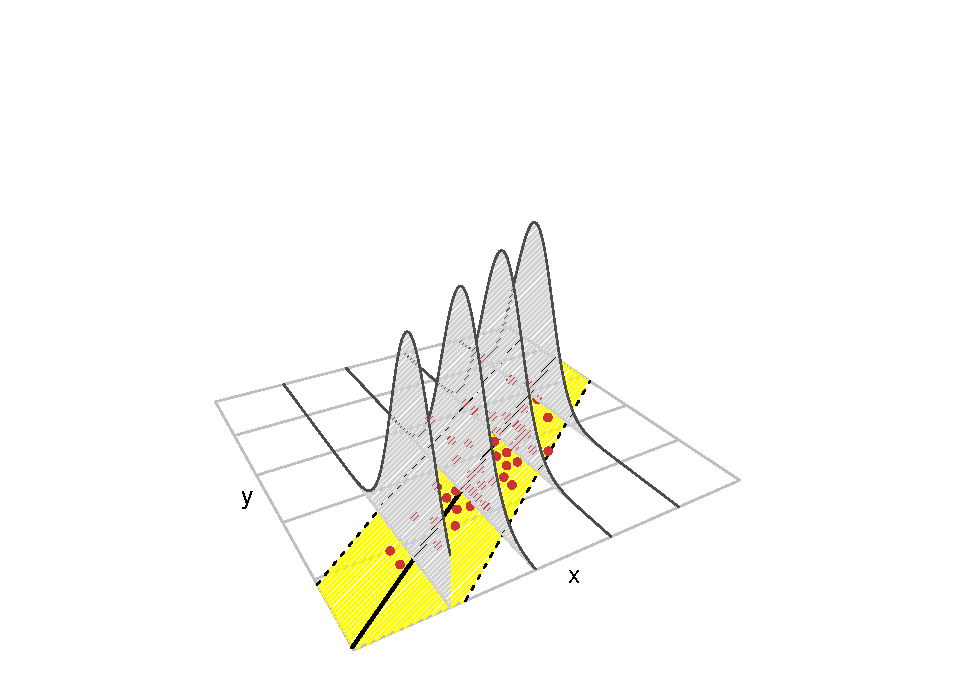
\includegraphics[width=0.6\linewidth]{Lab_5_files/figure-latex/unnamed-chunk-3-1} \end{center}

\begin{rmdinsight}
\begin{itemize}
\item
  Nicio ipoteză nu a fost făcută asupra repartiției lui \(X\) (poate fi
  sau deterministă sau aleatoare)
\item
  Modelul de regresie presupune că \textbf{\(Y\) este continuă} datorită
  normalității erorilor. În orice caz, \textbf{\(X\) poate fi o
  variabilă discretă}!
\end{itemize}
\end{rmdinsight}

Dat fiind un eșantion \((X_1,Y_1),\ldots,(X_n,Y_n)\) pentru variabilele
\(X\) și \(Y\) putem estima coeficienții necunoscuți \(\beta_0\) și
\(\beta_1\) minimizând \emph{suma abaterilor pătratice reziduale}
(\emph{Residual Sum of Squares} - RSS)

\[
\text{RSS}(\beta_0,\beta_1)=\sum_{i=1}^n(Y_i-\beta_0-\beta_1x_i)^2
\]

ceea ce conduce la

\[
\hat\beta_0=\bar{Y}-\hat\beta_1\bar{x},\quad \hat\beta_1=\frac{S_{xy}}{S_{xx}}=\frac{\sum_{i=1}^{n}{(x_i-\bar{x})}Y_i}{\sum_{i=1}^{n}{(x_i-\bar{x})^2}}
\]

unde folosim notațiile

\begin{itemize}
\item
  \(\bar{X}=\frac{1}{n}\sum_{i=1}^nX_i\) este \emph{media eșantionului}
\item
  \(S_{xx}=\sum_{i=1}^n(X_i-\bar{X})^2\) este \emph{suma abaterilor
  pătratice pentru \(X\)}
\item
  \(S_{yy}=\sum_{i=1}^n(Y_i-\bar{Y})^2\) este \emph{suma abaterilor
  pătratice pentru \(Y\)}
\item
  \(S_{xy}=\sum_{i=1}^n(X_i-\bar{X})(Y_i-\bar{Y})\) este \emph{suma
  produselor încrucișate}
\end{itemize}

Graficul functiei RSS pentru modelul \(y = -0.5 + 1.5x + e\):

\begin{center}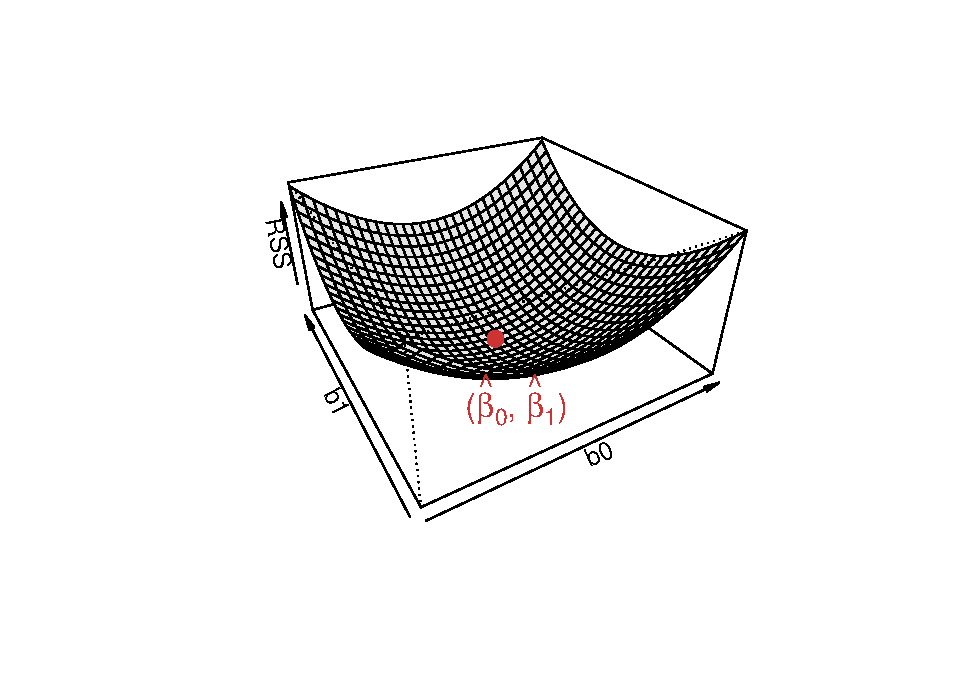
\includegraphics[width=0.7\linewidth]{Lab_5_files/figure-latex/unnamed-chunk-5-1} \end{center}

Odată ce avem estimatorii \((\hat\beta_0,\hat\beta_1)\) , putem defini:

\begin{itemize}
\tightlist
\item
  \emph{valorile prognozate} (\emph{fitted values})
  \(\hat Y_1,\ldots,\hat Y_n\) (valorile verticale pe dreapta de
  regresie), unde
\end{itemize}

\[
\hat Y_i=\hat\beta_0+\hat\beta_1x_i,\quad i=1,\ldots,n
\]

\begin{itemize}
\tightlist
\item
  \emph{reziduurile estimate} (\emph{estimated residuals})
  \(\hat \varepsilon_1,\ldots,\hat \varepsilon_n\) (distanțele verticale
  dintre punctele actuale \((X_i,Y_i)\) și cele prognozate
  \((X_i,\hat Y_i)\)), unde
\end{itemize}

\[
\hat\varepsilon_i=Y_i-\hat Y_i,\quad i=1,\ldots,n
\]

Estimatorul pentru \(\sigma^2\) este

\[
\hat{\sigma}^2 = \frac{RSS(\hat{\beta}_0,\hat{\beta}_1)}{n-2} = \frac{\sum_{i=1}^{n}\hat{\varepsilon}_i^2}{n-2}.
\]

\subsection{\texorpdfstring{Funcția \emph{lm()} din
R}{Funcția lm() din R}}\label{functia-lm-din-r}

Pentru a rula modelul de regresie liniară simplă în R se folosește
funcția \texttt{lm()} (\emph{linear model}). Funcția \texttt{lm()} are
două argumente esențiale: \texttt{formula} și \texttt{data}.

\begin{longtable}[]{@{}ll@{}}
\toprule
\begin{minipage}[b]{0.18\columnwidth}\raggedright\strut
Argument\strut
\end{minipage} & \begin{minipage}[b]{0.67\columnwidth}\raggedright\strut
Descriere\strut
\end{minipage}\tabularnewline
\midrule
\endhead
\begin{minipage}[t]{0.18\columnwidth}\raggedright\strut
\texttt{formula}\strut
\end{minipage} & \begin{minipage}[t]{0.67\columnwidth}\raggedright\strut
O formulă de forma \(y \sim x_1 + x_2 + \ldots\), unde \(y\) este
variabila răspuns (dependentă) iar \(x_1,x_2,\ldots\) sunt variabilele
explicative (independente). Dacă vrem să includem toate coloanele (cu
excepția lui \(y\)) ca variabile explicative putem folosi
\(y \sim .\)\strut
\end{minipage}\tabularnewline
\begin{minipage}[t]{0.18\columnwidth}\raggedright\strut
\texttt{data}\strut
\end{minipage} & \begin{minipage}[t]{0.67\columnwidth}\raggedright\strut
Este setul de date în format \texttt{data.frame} care conține coloanele
specificate de formulă.\strut
\end{minipage}\tabularnewline
\bottomrule
\end{longtable}

Următorul tabel conține corespondențe între codul \texttt{R} și
conceptele statistice asociate modelului de regresie:

\begin{longtable}[]{@{}ll@{}}
\toprule
\begin{minipage}[b]{0.49\columnwidth}\raggedright\strut
\texttt{R}\strut
\end{minipage} & \begin{minipage}[b]{0.45\columnwidth}\raggedright\strut
Concepte statistice\strut
\end{minipage}\tabularnewline
\midrule
\endhead
\begin{minipage}[t]{0.49\columnwidth}\raggedright\strut
\texttt{x}\strut
\end{minipage} & \begin{minipage}[t]{0.45\columnwidth}\raggedright\strut
Variabilele predictor \(X_1,\ldots,X_n\)\strut
\end{minipage}\tabularnewline
\begin{minipage}[t]{0.49\columnwidth}\raggedright\strut
\texttt{y}\strut
\end{minipage} & \begin{minipage}[t]{0.45\columnwidth}\raggedright\strut
Răspunsul \(Y_1,\ldots,Y_n\)\strut
\end{minipage}\tabularnewline
\begin{minipage}[t]{0.49\columnwidth}\raggedright\strut
\texttt{data\ \textless{}-\ data.frame(x\ =\ x,\ y\ =\ y)}\strut
\end{minipage} & \begin{minipage}[t]{0.45\columnwidth}\raggedright\strut
Eșantionul \((X_1,Y_1),\ldots,(X_n,Y_n)\)\strut
\end{minipage}\tabularnewline
\begin{minipage}[t]{0.49\columnwidth}\raggedright\strut
\texttt{model\ \textless{}-\ lm(y\ \textasciitilde{}\ x,\ data\ =\ data)}\strut
\end{minipage} & \begin{minipage}[t]{0.45\columnwidth}\raggedright\strut
Modelul de regresie liniară simplă\strut
\end{minipage}\tabularnewline
\begin{minipage}[t]{0.49\columnwidth}\raggedright\strut
\texttt{model\$coefficients}\strut
\end{minipage} & \begin{minipage}[t]{0.45\columnwidth}\raggedright\strut
Coeficienții \(\hat\beta_0,\hat\beta_1\)\strut
\end{minipage}\tabularnewline
\begin{minipage}[t]{0.49\columnwidth}\raggedright\strut
\texttt{model\$residuals}\strut
\end{minipage} & \begin{minipage}[t]{0.45\columnwidth}\raggedright\strut
Valorile reziduale \(\hat\varepsilon_1,\ldots,\hat\varepsilon_n\)\strut
\end{minipage}\tabularnewline
\begin{minipage}[t]{0.49\columnwidth}\raggedright\strut
\texttt{model\$fitted.values}\strut
\end{minipage} & \begin{minipage}[t]{0.45\columnwidth}\raggedright\strut
Valorile fitate \(\hat Y_1,\ldots,\hat Y_n\)\strut
\end{minipage}\tabularnewline
\begin{minipage}[t]{0.49\columnwidth}\raggedright\strut
\texttt{model\$df.residual}\strut
\end{minipage} & \begin{minipage}[t]{0.45\columnwidth}\raggedright\strut
Gradele de libertate \(n-2\)\strut
\end{minipage}\tabularnewline
\begin{minipage}[t]{0.49\columnwidth}\raggedright\strut
\texttt{summaryModel\ \textless{}-\ summary(model)}\strut
\end{minipage} & \begin{minipage}[t]{0.45\columnwidth}\raggedright\strut
Sumarul modelului de regresie liniară\strut
\end{minipage}\tabularnewline
\begin{minipage}[t]{0.49\columnwidth}\raggedright\strut
\texttt{summaryModel\$sigma}\strut
\end{minipage} & \begin{minipage}[t]{0.45\columnwidth}\raggedright\strut
Estimatorul \(\hat\sigma\)\strut
\end{minipage}\tabularnewline
\begin{minipage}[t]{0.49\columnwidth}\raggedright\strut
\texttt{summaryModel\$r.squared}\strut
\end{minipage} & \begin{minipage}[t]{0.45\columnwidth}\raggedright\strut
Coeficientul de determinare \(R^2\)\strut
\end{minipage}\tabularnewline
\begin{minipage}[t]{0.49\columnwidth}\raggedright\strut
\texttt{summaryModel\$fstatistic}\strut
\end{minipage} & \begin{minipage}[t]{0.45\columnwidth}\raggedright\strut
Testul lui Fisher \(F\)\strut
\end{minipage}\tabularnewline
\begin{minipage}[t]{0.49\columnwidth}\raggedright\strut
\texttt{anova(model)}\strut
\end{minipage} & \begin{minipage}[t]{0.45\columnwidth}\raggedright\strut
Tabelul ANOVA\strut
\end{minipage}\tabularnewline
\bottomrule
\end{longtable}

\section{Aplicație}\label{aplicatie}

\begin{rmdexercise}
Ne propunem să investigăm relația dintre volumul vânzărilor dintr-un
anumit produs (calculate în mii de unități) și bugetul (în milioane RON)
alocat pentru publicitatea la televizor. Pentru aceasta vom folosi setul
de date \href{dataIn/advertising.csv}{advertising} care conține
informații despre volumul vânzărilor și bugetul alocat publicității TV
în 200 de piețe de desfacere.
\end{rmdexercise}

Începem prin a înregistra setul de date

\begin{Shaded}
\begin{Highlighting}[]
\NormalTok{advertise =}\StringTok{ }\KeywordTok{read.csv}\NormalTok{(}\StringTok{"dataIn/advertising.csv"}\NormalTok{, }\DataTypeTok{row.names =} \DecValTok{1}\NormalTok{)}

\KeywordTok{summary}\NormalTok{(advertise)}
\NormalTok{       TV             radio          newspaper          sales      }
\NormalTok{ Min.   }\OperatorTok{:}\StringTok{  }\FloatTok{0.70}\NormalTok{   Min.   }\OperatorTok{:}\StringTok{ }\FloatTok{0.000}\NormalTok{   Min.   }\OperatorTok{:}\StringTok{  }\FloatTok{0.30}\NormalTok{   Min.   }\OperatorTok{:}\StringTok{ }\FloatTok{1.60}  
\NormalTok{ 1st Qu.}\OperatorTok{:}\StringTok{ }\FloatTok{74.38}\NormalTok{   1st Qu.}\OperatorTok{:}\StringTok{ }\FloatTok{9.975}\NormalTok{   1st Qu.}\OperatorTok{:}\StringTok{ }\FloatTok{12.75}\NormalTok{   1st Qu.}\OperatorTok{:}\FloatTok{10.38}  
\NormalTok{ Median }\OperatorTok{:}\FloatTok{149.75}\NormalTok{   Median }\OperatorTok{:}\FloatTok{22.900}\NormalTok{   Median }\OperatorTok{:}\StringTok{ }\FloatTok{25.75}\NormalTok{   Median }\OperatorTok{:}\FloatTok{12.90}  
\NormalTok{ Mean   }\OperatorTok{:}\FloatTok{147.04}\NormalTok{   Mean   }\OperatorTok{:}\FloatTok{23.264}\NormalTok{   Mean   }\OperatorTok{:}\StringTok{ }\FloatTok{30.55}\NormalTok{   Mean   }\OperatorTok{:}\FloatTok{14.02}  
\NormalTok{ 3rd Qu.}\OperatorTok{:}\FloatTok{218.82}\NormalTok{   3rd Qu.}\OperatorTok{:}\FloatTok{36.525}\NormalTok{   3rd Qu.}\OperatorTok{:}\StringTok{ }\FloatTok{45.10}\NormalTok{   3rd Qu.}\OperatorTok{:}\FloatTok{17.40}  
\NormalTok{ Max.   }\OperatorTok{:}\FloatTok{296.40}\NormalTok{   Max.   }\OperatorTok{:}\FloatTok{49.600}\NormalTok{   Max.   }\OperatorTok{:}\FloatTok{114.00}\NormalTok{   Max.   }\OperatorTok{:}\FloatTok{27.00}  
\end{Highlighting}
\end{Shaded}

și a ilustra grafic diagrama de împrăștiere

\begin{Shaded}
\begin{Highlighting}[]
\KeywordTok{plot}\NormalTok{(advertise}\OperatorTok{$}\NormalTok{TV, advertise}\OperatorTok{$}\NormalTok{sales, }
     \DataTypeTok{xlab =} \StringTok{"Publicitate TV"}\NormalTok{, }
     \DataTypeTok{ylab =} \StringTok{"Volum vanzari"}\NormalTok{, }
     \DataTypeTok{col =} \StringTok{"brown3"}\NormalTok{, }
     \DataTypeTok{pch =} \DecValTok{16}\NormalTok{, }
     \DataTypeTok{bty=}\StringTok{"n"}\NormalTok{)}
\end{Highlighting}
\end{Shaded}

\begin{center}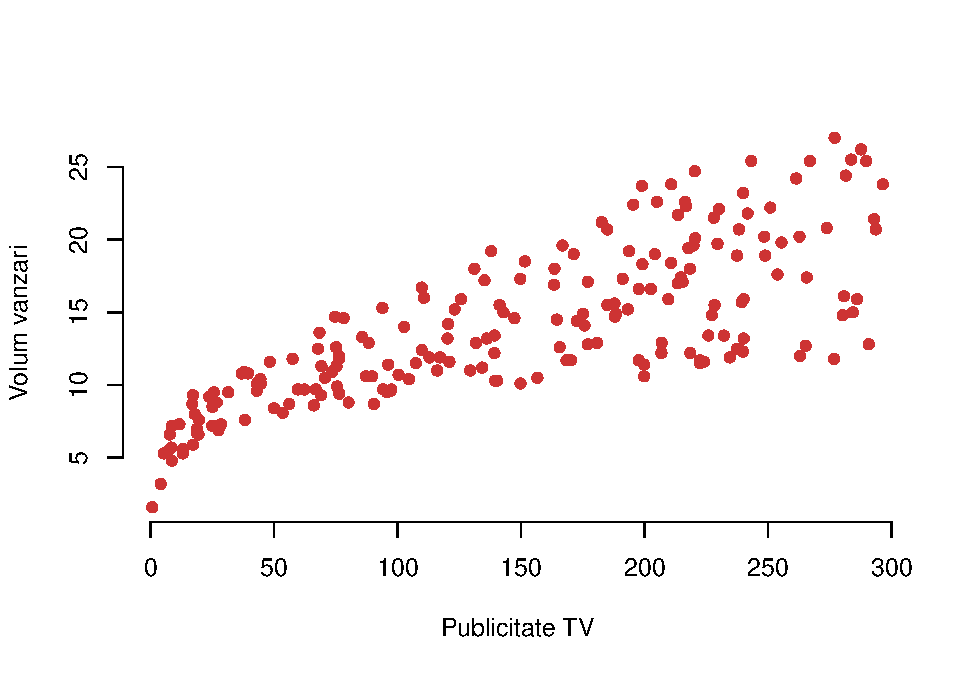
\includegraphics[width=0.8\linewidth]{Lab_5_files/figure-latex/unnamed-chunk-8-1} \end{center}

\subsection{Estimarea parametrilor}\label{estimarea-parametrilor}

Considerăm modelul de regresie \(Y = \beta_0 + \beta_1 X + \varepsilon\)
(unde \(X=\)\texttt{advertise\$TV} iar \(Y=\)\texttt{advertise\$sales}),
\(\varepsilon\sim \mathcal{N}(0,\sigma^2)\), a cărui parametrii sunt
\(\beta_0\), \(\beta_1\) și \(\sigma^2\).

Observăm că estimatorii parametrilor \(\beta_0\) și \(\beta_1\) sunt
dați de

\begin{Shaded}
\begin{Highlighting}[]
\CommentTok{# pentru b1}

\NormalTok{b1 =}\StringTok{ }\KeywordTok{cov}\NormalTok{(advertise}\OperatorTok{$}\NormalTok{TV, advertise}\OperatorTok{$}\NormalTok{sales)}\OperatorTok{/}\KeywordTok{var}\NormalTok{(advertise}\OperatorTok{$}\NormalTok{TV)}
\KeywordTok{cat}\NormalTok{(}\StringTok{"b1 = "}\NormalTok{, b1, }\StringTok{"}\CharTok{\textbackslash{}n}\StringTok{"}\NormalTok{)}
\NormalTok{b1 =}\StringTok{  }\FloatTok{0.04753664} 

\CommentTok{# sau }

\KeywordTok{sum}\NormalTok{((advertise}\OperatorTok{$}\NormalTok{TV}\OperatorTok{-}\KeywordTok{mean}\NormalTok{(advertise}\OperatorTok{$}\NormalTok{TV))}\OperatorTok{*}\NormalTok{(advertise}\OperatorTok{$}\NormalTok{sales))}\OperatorTok{/}
\StringTok{  }\KeywordTok{sum}\NormalTok{((advertise}\OperatorTok{$}\NormalTok{TV}\OperatorTok{-}\KeywordTok{mean}\NormalTok{(advertise}\OperatorTok{$}\NormalTok{TV))}\OperatorTok{^}\DecValTok{2}\NormalTok{)}
\NormalTok{[}\DecValTok{1}\NormalTok{] }\FloatTok{0.04753664}

\CommentTok{# pentru b0}

\NormalTok{b0 =}\StringTok{ }\KeywordTok{mean}\NormalTok{(advertise}\OperatorTok{$}\NormalTok{sales) }\OperatorTok{-}\StringTok{ }\NormalTok{b1}\OperatorTok{*}\KeywordTok{mean}\NormalTok{(advertise}\OperatorTok{$}\NormalTok{TV)}
\KeywordTok{cat}\NormalTok{(}\StringTok{"b0 = "}\NormalTok{, b0)}
\NormalTok{b0 =}\StringTok{  }\FloatTok{7.032594}
\end{Highlighting}
\end{Shaded}

sau folosind funcția \texttt{lm()}:

\begin{Shaded}
\begin{Highlighting}[]
\NormalTok{advertise_TV_model =}\StringTok{ }\KeywordTok{lm}\NormalTok{(sales}\OperatorTok{~}\NormalTok{TV, }\DataTypeTok{data =}\NormalTok{ advertise)}
\KeywordTok{names}\NormalTok{(advertise_TV_model)}
\NormalTok{ [}\DecValTok{1}\NormalTok{] }\StringTok{"coefficients"}  \StringTok{"residuals"}     \StringTok{"effects"}       \StringTok{"rank"}         
\NormalTok{ [}\DecValTok{5}\NormalTok{] }\StringTok{"fitted.values"} \StringTok{"assign"}        \StringTok{"qr"}            \StringTok{"df.residual"}  
\NormalTok{ [}\DecValTok{9}\NormalTok{] }\StringTok{"xlevels"}       \StringTok{"call"}          \StringTok{"terms"}         \StringTok{"model"}        
\end{Highlighting}
\end{Shaded}

\begin{Shaded}
\begin{Highlighting}[]
\NormalTok{advertise_TV_model}\OperatorTok{$}\NormalTok{coefficients}
\NormalTok{(Intercept)          TV }
 \FloatTok{7.03259355}  \FloatTok{0.04753664} 
\end{Highlighting}
\end{Shaded}

Graficul sumei abaterilor pătratice reziduale \(RSS\) este

\begin{center}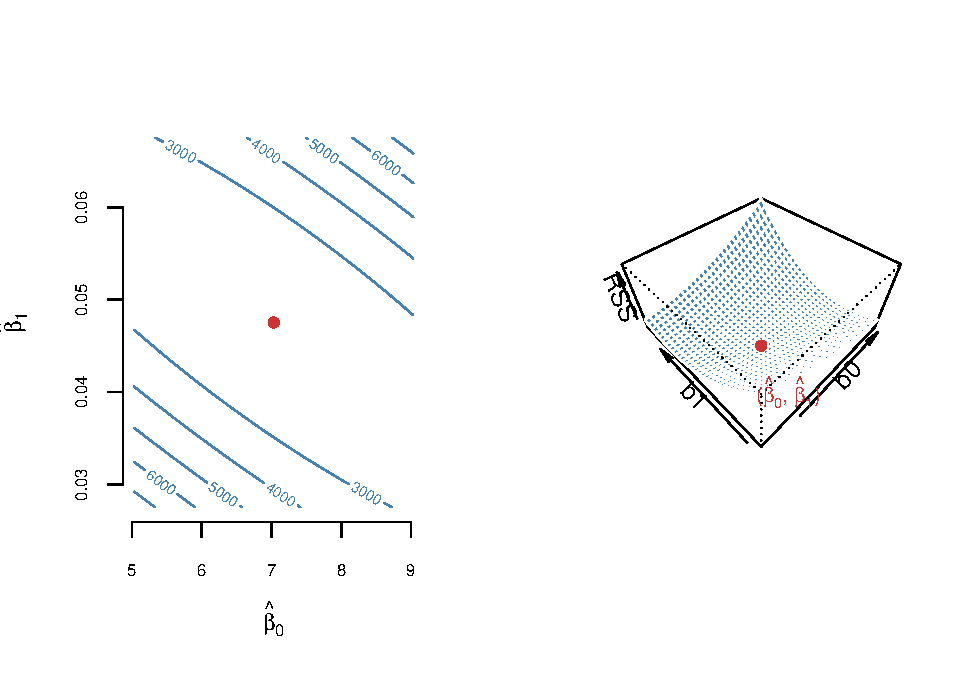
\includegraphics[width=0.8\linewidth]{Lab_5_files/figure-latex/unnamed-chunk-12-1} \end{center}

Dreapta de regresie (observăm că aceasta trece prin punctul de
coordonate \((\bar{x}, \bar{y})\)) este:

\begin{Shaded}
\begin{Highlighting}[]
\KeywordTok{plot}\NormalTok{(advertise}\OperatorTok{$}\NormalTok{TV, advertise}\OperatorTok{$}\NormalTok{sales, }
     \DataTypeTok{xlab =} \StringTok{"Publicitate TV"}\NormalTok{, }
     \DataTypeTok{ylab =} \StringTok{"Volumul vanzarilor"}\NormalTok{, }
     \DataTypeTok{col =} \StringTok{"brown3"}\NormalTok{, }
     \DataTypeTok{pch =} \DecValTok{20}\NormalTok{, }
     \DataTypeTok{bty=}\StringTok{"n"}\NormalTok{, }
     \DataTypeTok{main =} \KeywordTok{paste}\NormalTok{(}\StringTok{"y = "}\NormalTok{, }\KeywordTok{format}\NormalTok{(b0, }\DataTypeTok{digits =} \DecValTok{4}\NormalTok{), }\StringTok{" + "}\NormalTok{, }
                  \KeywordTok{format}\NormalTok{(b1, }\DataTypeTok{digits =} \DecValTok{4}\NormalTok{), }\StringTok{" x"}\NormalTok{))}

\KeywordTok{abline}\NormalTok{(}\DataTypeTok{a =}\NormalTok{ b0, }\DataTypeTok{b =}\NormalTok{ b1, }\DataTypeTok{col =} \StringTok{"royalblue"}\NormalTok{, }\DataTypeTok{lwd =} \DecValTok{2}\NormalTok{)}
\KeywordTok{points}\NormalTok{(}\KeywordTok{mean}\NormalTok{(advertise}\OperatorTok{$}\NormalTok{TV), }\KeywordTok{mean}\NormalTok{(advertise}\OperatorTok{$}\NormalTok{sales), }
       \DataTypeTok{pch =} \DecValTok{16}\NormalTok{, }
       \DataTypeTok{col =} \StringTok{"dark green"}\NormalTok{, }
       \DataTypeTok{cex =} \FloatTok{1.2}\NormalTok{)}
\KeywordTok{text}\NormalTok{(}\KeywordTok{mean}\NormalTok{(advertise}\OperatorTok{$}\NormalTok{TV), }\KeywordTok{mean}\NormalTok{(advertise}\OperatorTok{$}\NormalTok{sales)}\OperatorTok{-}\FloatTok{1.3}\NormalTok{, }
     \DataTypeTok{col =} \StringTok{"dark green"}\NormalTok{, }\DataTypeTok{cex =} \FloatTok{1.2}\NormalTok{, }
     \DataTypeTok{labels =} \KeywordTok{expression}\NormalTok{(}\KeywordTok{paste}\NormalTok{(}\StringTok{"("}\NormalTok{, }\KeywordTok{bar}\NormalTok{(x), }\StringTok{","}\NormalTok{, }\KeywordTok{bar}\NormalTok{(y),}\StringTok{")"}\NormalTok{)))}
\end{Highlighting}
\end{Shaded}

\begin{center}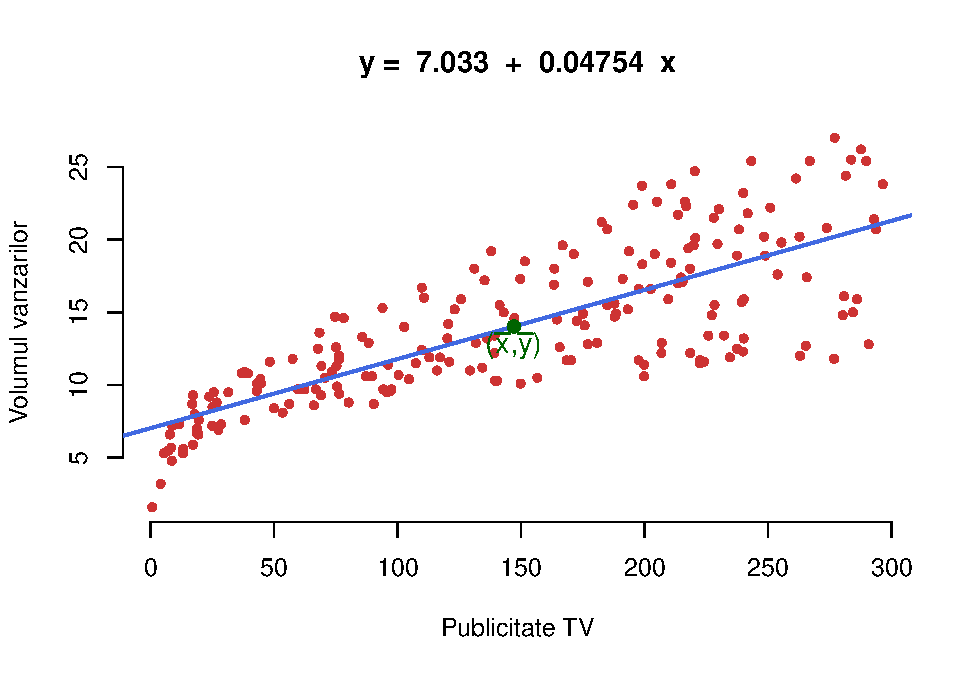
\includegraphics[width=0.8\linewidth]{Lab_5_files/figure-latex/unnamed-chunk-13-1} \end{center}

De asemenea pentru calculul estimatorului lui \(\sigma\)
(\(\hat{\sigma}\)) avem

\begin{Shaded}
\begin{Highlighting}[]
\NormalTok{n =}\StringTok{ }\KeywordTok{length}\NormalTok{(advertise}\OperatorTok{$}\NormalTok{sales)}
\NormalTok{e_hat =}\StringTok{ }\NormalTok{advertise}\OperatorTok{$}\NormalTok{sales }\OperatorTok{-}\StringTok{ }\NormalTok{(b0}\OperatorTok{+}\NormalTok{b1}\OperatorTok{*}\NormalTok{advertise}\OperatorTok{$}\NormalTok{TV)}

\NormalTok{rss =}\StringTok{ }\KeywordTok{sum}\NormalTok{(e_hat}\OperatorTok{^}\DecValTok{2}\NormalTok{)}
\CommentTok{# sau folosind comanda deviance(advertise_TV_model)}

\NormalTok{sigma_hat =}\StringTok{ }\KeywordTok{sqrt}\NormalTok{(rss}\OperatorTok{/}\NormalTok{(n}\OperatorTok{-}\DecValTok{2}\NormalTok{))}
\NormalTok{sigma_hat}
\NormalTok{[}\DecValTok{1}\NormalTok{] }\FloatTok{3.258656}
\end{Highlighting}
\end{Shaded}

sau cu ajutorul funcției \texttt{lm()}

\begin{Shaded}
\begin{Highlighting}[]
\KeywordTok{sqrt}\NormalTok{(}\KeywordTok{deviance}\NormalTok{(advertise_TV_model)}\OperatorTok{/}\KeywordTok{df.residual}\NormalTok{(advertise_TV_model))}
\NormalTok{[}\DecValTok{1}\NormalTok{] }\FloatTok{3.258656}
\end{Highlighting}
\end{Shaded}

sau încă aplicând funcția \texttt{summary()}

\begin{Shaded}
\begin{Highlighting}[]
\NormalTok{advertise_TV_model_summary =}\StringTok{ }\KeywordTok{summary}\NormalTok{(advertise_TV_model)}

\NormalTok{advertise_TV_model_summary}\OperatorTok{$}\NormalTok{sigma}
\NormalTok{[}\DecValTok{1}\NormalTok{] }\FloatTok{3.258656}
\end{Highlighting}
\end{Shaded}

\subsection{Intervale de încredere pentru
parametrii}\label{intervale-de-incredere-pentru-parametrii}

Repartițiile lui \(\hat\beta_0\) și \(\hat\beta_1\) sunt

\[
\hat\beta_0\sim\mathcal{N}\left(\beta_0,\mathrm{SE}(\hat\beta_0)^2\right),\quad\hat\beta_1\sim\mathcal{N}\left(\beta_1,\mathrm{SE}(\hat\beta_1)^2\right)
\]

unde

\[
\mathrm{SE}(\hat\beta_0)^2=\sigma^2\left[\frac{1}{n}+\frac{\bar x^2}{\sum_{i=1}^{n}(x_i-\bar{x})^2}\right]=\sigma^2\left[\frac{1}{n}+\frac{\bar x^2}{S_{xx}}\right],\quad  \mathrm{SE}(\hat\beta_1)^2= \frac{\sigma^2}{\sum_{i=1}^{n}(x_i-\bar{x})^2} = \frac{\sigma^2}{S_{xx}}.
\]

Folosind estimatorul \(\hat\sigma^2\) pentru \(\sigma^2\) obținem că

\[
\frac{\hat\beta_0-\beta_0}{\hat{\mathrm{SE}}(\hat\beta_0)}\sim t_{n-2},\quad\frac{\hat\beta_1-\beta_1}{\hat{\mathrm{SE}}(\hat\beta_1)}\sim t_{n-2}
\]

unde

\[
\hat{\mathrm{SE}}(\hat\beta_0)^2=\hat \sigma^2\left[\frac{1}{n}+\frac{\bar x^2}{\sum_{i=1}^{n}(x_i-\bar{x})^2}\right]=\hat \sigma^2\left[\frac{1}{n}+\frac{\bar x^2}{S_{xx}}\right],\quad \hat{\mathrm{SE}}(\hat\beta_1)^2=\frac{\hat \sigma^2}{\sum_{i=1}^{n}(x_i-\bar{x})^2} = \frac{\hat \sigma^2}{S_{xx}}
\]

prin urmare, intervalele de încredere de nivel \(1-\alpha\) pentru
\(\beta_0\) și \(\beta_1\) sunt

\[
IC = \left(\hat\beta_j\pm\hat{\mathrm{SE}}(\hat\beta_j)t_{n-2;1-\alpha/2}\right),\quad j=0,1.
\]

În R putem calcula aceste intervale de încredere folosind comenzile

\begin{Shaded}
\begin{Highlighting}[]
\NormalTok{alpha =}\StringTok{ }\FloatTok{0.05}

\CommentTok{# trebuie avut grija ca functia var si sd se calculeaza }
\CommentTok{# impartind la (n-1) si nu la n !!!}

\NormalTok{se_b0 =}\StringTok{ }\KeywordTok{sqrt}\NormalTok{(sigma_hat}\OperatorTok{^}\DecValTok{2}\OperatorTok{*}\NormalTok{(}\DecValTok{1}\OperatorTok{/}\NormalTok{n}\OperatorTok{+}\KeywordTok{mean}\NormalTok{(advertise}\OperatorTok{$}\NormalTok{TV)}\OperatorTok{^}\DecValTok{2}\OperatorTok{/}\NormalTok{((n}\OperatorTok{-}\DecValTok{1}\NormalTok{)}\OperatorTok{*}\KeywordTok{var}\NormalTok{(advertise}\OperatorTok{$}\NormalTok{TV))))}
\NormalTok{se_b1 =}\StringTok{ }\KeywordTok{sqrt}\NormalTok{(sigma_hat}\OperatorTok{^}\DecValTok{2}\OperatorTok{/}\NormalTok{((n}\OperatorTok{-}\DecValTok{1}\NormalTok{)}\OperatorTok{*}\KeywordTok{var}\NormalTok{(advertise}\OperatorTok{$}\NormalTok{TV)))}

\NormalTok{lw_b0 =}\StringTok{ }\NormalTok{b0 }\OperatorTok{-}\StringTok{ }\KeywordTok{qt}\NormalTok{(}\DecValTok{1}\OperatorTok{-}\NormalTok{alpha}\OperatorTok{/}\DecValTok{2}\NormalTok{, n}\OperatorTok{-}\DecValTok{2}\NormalTok{)}\OperatorTok{*}\NormalTok{se_b0}
\NormalTok{up_b0 =}\StringTok{ }\NormalTok{b0 }\OperatorTok{+}\StringTok{ }\KeywordTok{qt}\NormalTok{(}\DecValTok{1}\OperatorTok{-}\NormalTok{alpha}\OperatorTok{/}\DecValTok{2}\NormalTok{, n}\OperatorTok{-}\DecValTok{2}\NormalTok{)}\OperatorTok{*}\NormalTok{se_b0}

\KeywordTok{cat}\NormalTok{(}\StringTok{"CI pentru b0 este ("}\NormalTok{, lw_b0, }\StringTok{", "}\NormalTok{, up_b0, }\StringTok{")}\CharTok{\textbackslash{}n}\StringTok{"}\NormalTok{)}
\NormalTok{CI pentru b0 }\KeywordTok{este}\NormalTok{ ( }\FloatTok{6.129719}\NormalTok{ ,  }\FloatTok{7.935468}\NormalTok{ )}

\NormalTok{lw_b1 =}\StringTok{ }\NormalTok{b1 }\OperatorTok{-}\StringTok{ }\KeywordTok{qt}\NormalTok{(}\DecValTok{1}\OperatorTok{-}\NormalTok{alpha}\OperatorTok{/}\DecValTok{2}\NormalTok{, n}\OperatorTok{-}\DecValTok{2}\NormalTok{)}\OperatorTok{*}\NormalTok{se_b1}
\NormalTok{up_b1 =}\StringTok{ }\NormalTok{b1 }\OperatorTok{+}\StringTok{ }\KeywordTok{qt}\NormalTok{(}\DecValTok{1}\OperatorTok{-}\NormalTok{alpha}\OperatorTok{/}\DecValTok{2}\NormalTok{, n}\OperatorTok{-}\DecValTok{2}\NormalTok{)}\OperatorTok{*}\NormalTok{se_b1}
  
\KeywordTok{cat}\NormalTok{(}\StringTok{"CI pentru b1 este ("}\NormalTok{, lw_b1, }\StringTok{", "}\NormalTok{, up_b1, }\StringTok{")"}\NormalTok{)}
\NormalTok{CI pentru b1 }\KeywordTok{este}\NormalTok{ ( }\FloatTok{0.04223072}\NormalTok{ ,  }\FloatTok{0.05284256}\NormalTok{ )}
\end{Highlighting}
\end{Shaded}

Același rezultat se obține apelând funcția \texttt{confint()} :

\begin{Shaded}
\begin{Highlighting}[]
\KeywordTok{confint}\NormalTok{(advertise_TV_model)}
                 \FloatTok{2.5} \OperatorTok
\NormalTok{(Intercept) }\FloatTok{6.12971927} \FloatTok{7.93546783}
\NormalTok{TV          }\FloatTok{0.04223072} \FloatTok{0.05284256}
\end{Highlighting}
\end{Shaded}

Observăm că în absența unui buget de publicitate TV, volumul vânzărilor
se încadrează în medie între \(6130\) și \(7940\) de unități. Mai mult,
pentru fiecare creștere a bugetului pentru publicitatea TV cu \(1000\)
de RON obținem o creștere, în medie, a vânzărilor între \(42\) și \(53\)
de unități.

Putem construi și o regiune de încredere de nivel de încredere
\(1-\alpha\) pentru vectorul \(\boldsymbol{\beta} = (\beta_0, \beta_1)\)
plecând de la repartiția bidimensională a vectorului
\(\boldsymbol{\hat \beta} = (\hat \beta_0, \hat \beta_1)^\intercal\). În
cazul modelului condițional normal avem că
\(\boldsymbol{\hat \beta}\sim\mathcal{N}(\boldsymbol{\beta}, \sigma^2 V)\)
unde

\[
  V = \frac{1}{\sigma^2}\begin{pmatrix}Var(\hat \beta_0) & Cov(\hat \beta_0, \hat \beta_1)\\ Cov(\hat \beta_0, \hat \beta_1) & Var(\hat \beta_1)\end{pmatrix} = \frac{1}{\sum_{i = 1}^{n}(x_i - \bar x)}\begin{pmatrix}\frac{\sum_{i = 1}^{n}x_i^2}{n} & -\bar x\\ -\bar x & 1\end{pmatrix}
\]

și cum

\[
\frac{1}{2\hat \sigma^2}\left(\boldsymbol{\hat \beta} - \boldsymbol{\beta}\right)^\intercal V^{-1} \left(\boldsymbol{\hat \beta} - \boldsymbol{\beta}\right) \sim F_{2, n-2}
\]

găsim că regiunea de încredere este

\[
  RC(\beta_0, \beta_1) = \left\{\frac{1}{2\hat\sigma^2}\left[n(\hat\beta_0 - \beta_0)^2 + 2n\bar x(\hat\beta_0 - \beta_0)(\hat\beta_1 - \beta_1) + (\hat\beta_1 - \beta_1)^2\sum_{i=1}^{n}x_i^2\right]\leq f^{1-\alpha}_{2,n-2}\right\}
\]

\begin{Shaded}
\begin{Highlighting}[]
\KeywordTok{library}\NormalTok{(ellipse)}
\KeywordTok{library}\NormalTok{(car)}

\KeywordTok{par}\NormalTok{(}\DataTypeTok{bty =} \StringTok{"n"}\NormalTok{)}

\CommentTok{# trasam regiunea de incredere}
\KeywordTok{confidenceEllipse}\NormalTok{(advertise_TV_model,}
                  \DataTypeTok{xlab =} \KeywordTok{expression}\NormalTok{(}\KeywordTok{hat}\NormalTok{(beta[}\DecValTok{0}\NormalTok{])), }
                  \DataTypeTok{ylab =} \KeywordTok{expression}\NormalTok{(}\KeywordTok{hat}\NormalTok{(beta[}\DecValTok{1}\NormalTok{])),}
                  \DataTypeTok{col =} \StringTok{"grey30"}\NormalTok{) }

\KeywordTok{points}\NormalTok{(}\KeywordTok{coef}\NormalTok{(advertise_TV_model)[}\DecValTok{1}\NormalTok{], }\KeywordTok{coef}\NormalTok{(advertise_TV_model)[}\DecValTok{2}\NormalTok{], }
       \DataTypeTok{pch =} \DecValTok{18}\NormalTok{, }\DataTypeTok{col =} \StringTok{"brown3"}\NormalTok{,}
       \DataTypeTok{cex =} \DecValTok{2}\NormalTok{)}

\CommentTok{# trasam intervalele de incredere}
\KeywordTok{abline}\NormalTok{(}\DataTypeTok{v =} \KeywordTok{confint}\NormalTok{(advertise_TV_model)[}\DecValTok{1}\NormalTok{,], }\DataTypeTok{lty =} \DecValTok{2}\NormalTok{)}
\KeywordTok{abline}\NormalTok{(}\DataTypeTok{h =} \KeywordTok{confint}\NormalTok{(advertise_TV_model)[}\DecValTok{2}\NormalTok{,], }\DataTypeTok{lty =} \DecValTok{2}\NormalTok{)}
\end{Highlighting}
\end{Shaded}

\begin{center}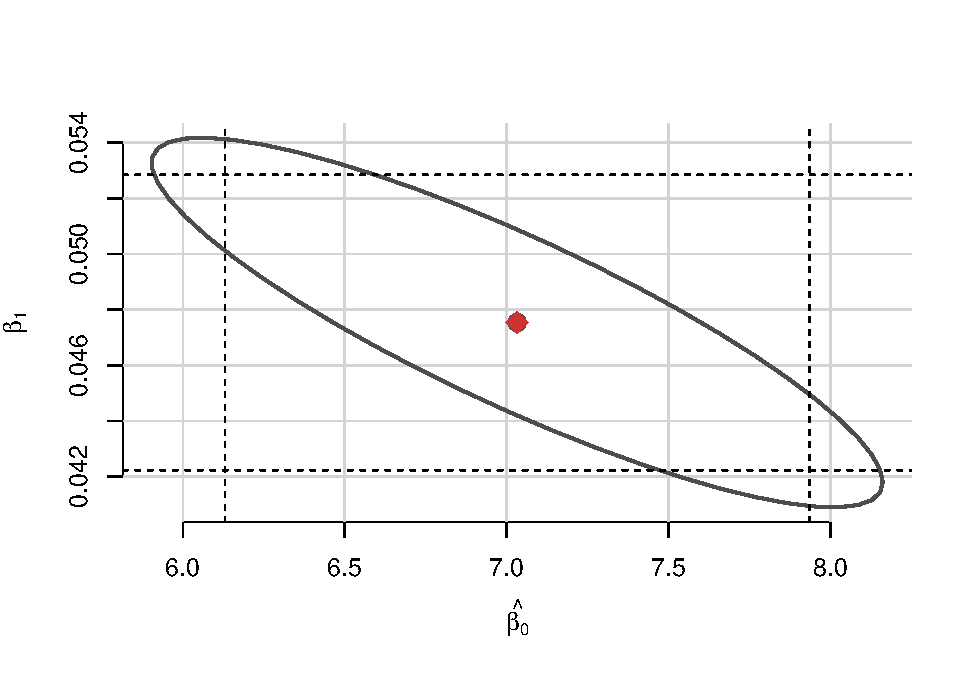
\includegraphics[width=0.8\linewidth]{Lab_5_files/figure-latex/unnamed-chunk-19-1} \end{center}

\subsection{ANOVA pentru regresie}\label{anova-pentru-regresie}

Este predictorul \(X\) folositor în prezicerea răspunsului \(Y\) ? Vrem
să testăm ipoteza nulă \(H_0:\;\beta_1=0\).

Introducem următoarele \emph{sume de abateri pătratice}:

\begin{itemize}
\item
  \(SS_T=\sum_{i=1}^n\left(Y_i-\bar Y\right)^2\), \textbf{suma totală a
  abaterilor pătratice} (variația totală a lui \(Y_1,\ldots,Y_n\)).
\item
  \(SS_{reg}=\sum_{i=1}^n\left(\hat Y_i-\bar Y\right)^2\), \textbf{suma
  abaterilor pătratice de regresie} (variabilitatea explicată de dreapta
  de regresie)
\item
  \(RSS=\sum_{i=1}^n\left(Y_i-\hat Y_i\right)^2\), \textbf{suma
  abaterilor pătratice reziduale}
\end{itemize}

Avem următoarea descompunere ANOVA

\[
\underbrace{SS_T}_{\text{Variația lui }Y_i} = \underbrace{SS_{reg}}_{\text{Variația lui }\hat Y_i} + \underbrace{RSS}_{\text{Variația lui }\hat \varepsilon_i} 
\]

și tabelul ANOVA corespunzător

\begin{longtable}[]{@{}llllll@{}}
\toprule
& Df & SS & MS & \(F\) & \(p\)-value\tabularnewline
\midrule
\endhead
Predictor & \(1\) & \(SS_{reg}\) & \(\frac{SS_{reg}}{1}\) &
\(\frac{SS_{reg}/1}{RSS/(n-2)}\) & \(p\)\tabularnewline
Residuuri & \(n - 2\) & \(RSS\) & \(\frac{RSS}{n-2}\) & &\tabularnewline
\bottomrule
\end{longtable}

Descompunerea ANOVA pentru problema noastră poate fi ilustrată astfel:

\begin{enumerate}
\def\labelenumi{\alph{enumi})}
\tightlist
\item
  \emph{suma abaterilor pătratice totală}:
\end{enumerate}

\begin{Shaded}
\begin{Highlighting}[]
\KeywordTok{plot}\NormalTok{(advertise}\OperatorTok{$}\NormalTok{TV, advertise}\OperatorTok{$}\NormalTok{sales, }\DataTypeTok{pch =} \DecValTok{20}\NormalTok{, }\DataTypeTok{type =} \StringTok{"n"}\NormalTok{,}
     \DataTypeTok{main =} \KeywordTok{paste}\NormalTok{(}\StringTok{"SST ="}\NormalTok{, }\KeywordTok{round}\NormalTok{(}\KeywordTok{sum}\NormalTok{((advertise}\OperatorTok{$}\NormalTok{sales }\OperatorTok{-}\StringTok{ }
\StringTok{                                        }\KeywordTok{mean}\NormalTok{(advertise}\OperatorTok{$}\NormalTok{sales))}\OperatorTok{^}\DecValTok{2}\NormalTok{), }\DecValTok{2}\NormalTok{)), }
     \DataTypeTok{col.main =} \StringTok{"brown4"}\NormalTok{, }
     \DataTypeTok{xlab =} \StringTok{"Publicitate TV"}\NormalTok{, }
     \DataTypeTok{ylab =} \StringTok{"Volumul vanzarilor"}\NormalTok{, }
     \DataTypeTok{bty =} \StringTok{"n"}\NormalTok{)}

\KeywordTok{abline}\NormalTok{(advertise_TV_model}\OperatorTok{$}\NormalTok{coefficients, }\DataTypeTok{col =} \StringTok{"royalblue"}\NormalTok{, }\DataTypeTok{lwd =} \DecValTok{2}\NormalTok{)}
\KeywordTok{abline}\NormalTok{(}\DataTypeTok{h =} \KeywordTok{mean}\NormalTok{(advertise}\OperatorTok{$}\NormalTok{sales), }\DataTypeTok{col =} \StringTok{"brown2"}\NormalTok{, }\DataTypeTok{lty =} \DecValTok{2}\NormalTok{, }\DataTypeTok{lwd =} \DecValTok{2}\NormalTok{)}

\KeywordTok{segments}\NormalTok{(}\DataTypeTok{x0 =}\NormalTok{ advertise}\OperatorTok{$}\NormalTok{TV, }\DataTypeTok{y0 =} \KeywordTok{mean}\NormalTok{(advertise}\OperatorTok{$}\NormalTok{sales), }
         \DataTypeTok{x1 =}\NormalTok{ advertise}\OperatorTok{$}\NormalTok{TV, }\DataTypeTok{y1 =}\NormalTok{ advertise}\OperatorTok{$}\NormalTok{sales, }
         \DataTypeTok{col =} \StringTok{"grey50"}\NormalTok{, }\DataTypeTok{lwd =} \DecValTok{1}\NormalTok{, }\DataTypeTok{lty =} \DecValTok{2}\NormalTok{)}

\KeywordTok{legend}\NormalTok{(}\StringTok{"topleft"}\NormalTok{, }
       \DataTypeTok{legend =} \KeywordTok{expression}\NormalTok{(}\StringTok{"Dreapta de regresie"}\NormalTok{, }\StringTok{"Media esantionului "} \OperatorTok{*}\StringTok{ }\KeywordTok{bar}\NormalTok{(Y),}
\NormalTok{                                      (Y[i] }\OperatorTok{-}\StringTok{ }\KeywordTok{bar}\NormalTok{(Y))}\OperatorTok{^}\DecValTok{2}\NormalTok{), }
       \DataTypeTok{lwd =} \KeywordTok{c}\NormalTok{(}\DecValTok{2}\NormalTok{, }\DecValTok{2}\NormalTok{, }\DecValTok{2}\NormalTok{),}
       \DataTypeTok{col =} \KeywordTok{c}\NormalTok{(}\StringTok{"royalblue"}\NormalTok{, }\StringTok{"brown2"}\NormalTok{, }\StringTok{"grey50"}\NormalTok{), }
       \DataTypeTok{lty =} \KeywordTok{c}\NormalTok{(}\DecValTok{1}\NormalTok{, }\DecValTok{2}\NormalTok{, }\DecValTok{2}\NormalTok{), }
       \DataTypeTok{bty =} \StringTok{"n"}\NormalTok{)}

\KeywordTok{points}\NormalTok{(advertise}\OperatorTok{$}\NormalTok{TV, advertise}\OperatorTok{$}\NormalTok{sales, }\DataTypeTok{pch =} \DecValTok{20}\NormalTok{, }\DataTypeTok{col =} \StringTok{"brown3"}\NormalTok{)}
\end{Highlighting}
\end{Shaded}

\begin{center}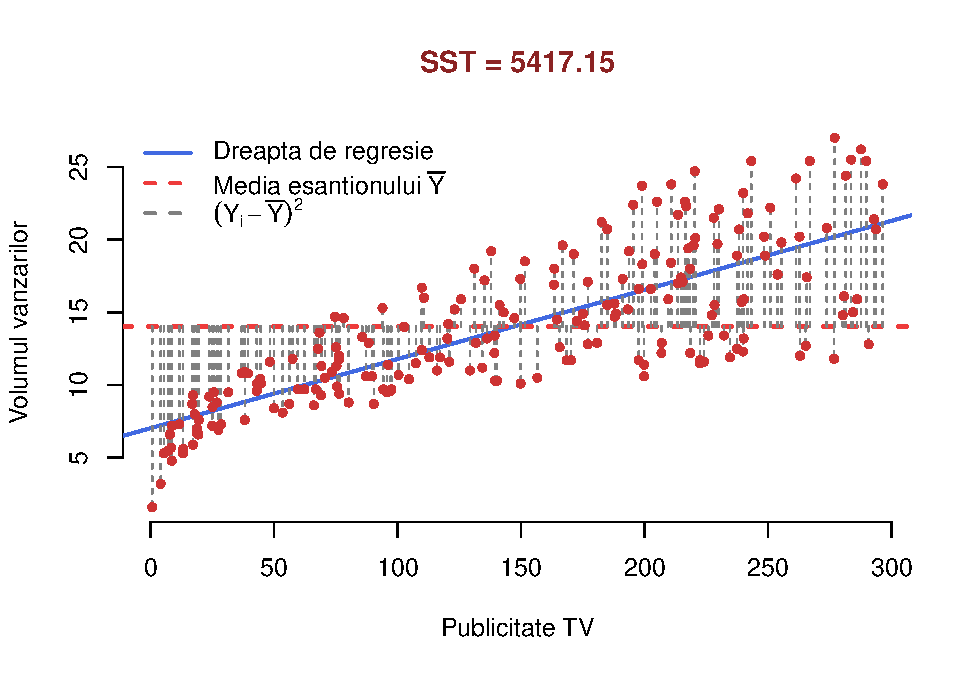
\includegraphics[width=0.8\linewidth]{Lab_5_files/figure-latex/unnamed-chunk-20-1} \end{center}

\begin{enumerate}
\def\labelenumi{\alph{enumi})}
\setcounter{enumi}{1}
\tightlist
\item
  \emph{suma abaterilor pătratice de regresie}
\end{enumerate}

\begin{Shaded}
\begin{Highlighting}[]
\KeywordTok{plot}\NormalTok{(advertise}\OperatorTok{$}\NormalTok{TV, advertise}\OperatorTok{$}\NormalTok{sales, }\DataTypeTok{pch =} \DecValTok{20}\NormalTok{, }\DataTypeTok{type =} \StringTok{"n"}\NormalTok{,}
     \DataTypeTok{main =} \KeywordTok{paste}\NormalTok{(}\StringTok{"SSreg ="}\NormalTok{, }
                  \KeywordTok{round}\NormalTok{(}\KeywordTok{sum}\NormalTok{((advertise_TV_model}\OperatorTok{$}\NormalTok{fitted.values }\OperatorTok{-}\StringTok{ }
\StringTok{                               }\KeywordTok{mean}\NormalTok{(advertise}\OperatorTok{$}\NormalTok{sales))}\OperatorTok{^}\DecValTok{2}\NormalTok{), }\DecValTok{2}\NormalTok{)), }
     \DataTypeTok{col.main =} \StringTok{"forestgreen"}\NormalTok{, }
     \DataTypeTok{xlab =} \StringTok{"Publicitate TV"}\NormalTok{, }
     \DataTypeTok{ylab =} \StringTok{"Volumul vanzarilor"}\NormalTok{, }
     \DataTypeTok{bty =} \StringTok{"n"}\NormalTok{)}

\KeywordTok{abline}\NormalTok{(advertise_TV_model}\OperatorTok{$}\NormalTok{coefficients, }\DataTypeTok{col =} \StringTok{"royalblue"}\NormalTok{, }\DataTypeTok{lwd =} \DecValTok{2}\NormalTok{)}
\KeywordTok{abline}\NormalTok{(}\DataTypeTok{h =} \KeywordTok{mean}\NormalTok{(advertise}\OperatorTok{$}\NormalTok{sales), }\DataTypeTok{col =} \StringTok{"brown2"}\NormalTok{, }\DataTypeTok{lty =} \DecValTok{2}\NormalTok{, }\DataTypeTok{lwd =} \DecValTok{2}\NormalTok{)}

\KeywordTok{segments}\NormalTok{(}\DataTypeTok{x0 =}\NormalTok{ advertise}\OperatorTok{$}\NormalTok{TV, }\DataTypeTok{y0 =} \KeywordTok{mean}\NormalTok{(advertise}\OperatorTok{$}\NormalTok{sales), }
         \DataTypeTok{x1 =}\NormalTok{ advertise}\OperatorTok{$}\NormalTok{TV, }\DataTypeTok{y1 =}\NormalTok{ advertise_TV_model}\OperatorTok{$}\NormalTok{fitted.values, }
         \DataTypeTok{col =} \StringTok{"forestgreen"}\NormalTok{, }\DataTypeTok{lwd =} \DecValTok{1}\NormalTok{, }\DataTypeTok{lty =} \DecValTok{2}\NormalTok{)}

\KeywordTok{points}\NormalTok{(advertise}\OperatorTok{$}\NormalTok{TV, advertise_TV_model}\OperatorTok{$}\NormalTok{fitted.values, }\DataTypeTok{pch =} \DecValTok{20}\NormalTok{, }\DataTypeTok{col =} \StringTok{"forestgreen"}\NormalTok{)}

\KeywordTok{legend}\NormalTok{(}\StringTok{"topleft"}\NormalTok{, }
       \DataTypeTok{legend =} \KeywordTok{expression}\NormalTok{(}\StringTok{"Dreapta de regresie"}\NormalTok{, }\StringTok{"Media esantionului "} \OperatorTok{*}\StringTok{ }\KeywordTok{bar}\NormalTok{(Y),}
\NormalTok{                                      (}\KeywordTok{hat}\NormalTok{(Y)[i] }\OperatorTok{-}\StringTok{ }\KeywordTok{bar}\NormalTok{(Y))}\OperatorTok{^}\DecValTok{2}\NormalTok{), }
       \DataTypeTok{lwd =} \KeywordTok{c}\NormalTok{(}\DecValTok{2}\NormalTok{, }\DecValTok{2}\NormalTok{, }\DecValTok{2}\NormalTok{),}
       \DataTypeTok{col =} \KeywordTok{c}\NormalTok{(}\StringTok{"royalblue"}\NormalTok{, }\StringTok{"brown2"}\NormalTok{, }\StringTok{"forestgreen"}\NormalTok{), }
       \DataTypeTok{lty =} \KeywordTok{c}\NormalTok{(}\DecValTok{1}\NormalTok{, }\DecValTok{2}\NormalTok{, }\DecValTok{2}\NormalTok{), }
       \DataTypeTok{bty =} \StringTok{"n"}\NormalTok{)}

\KeywordTok{points}\NormalTok{(advertise}\OperatorTok{$}\NormalTok{TV, advertise}\OperatorTok{$}\NormalTok{sales, }\DataTypeTok{pch =} \DecValTok{20}\NormalTok{, }\DataTypeTok{col =} \StringTok{"brown3"}\NormalTok{)}
\end{Highlighting}
\end{Shaded}

\begin{center}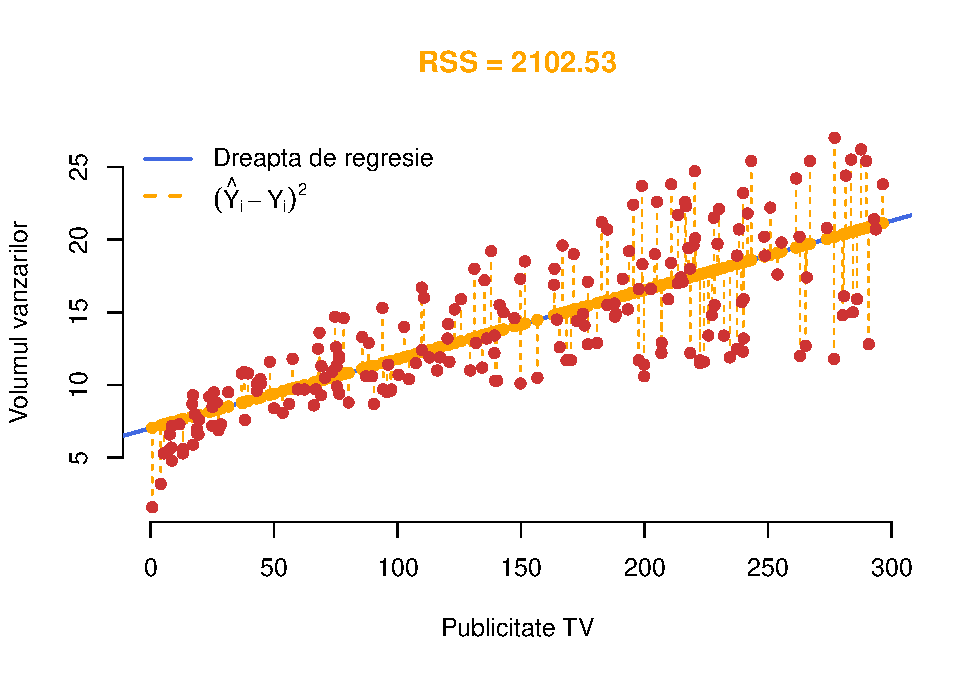
\includegraphics[width=0.8\linewidth]{Lab_5_files/figure-latex/unnamed-chunk-21-1} \end{center}

\begin{enumerate}
\def\labelenumi{\alph{enumi})}
\setcounter{enumi}{2}
\tightlist
\item
  \emph{suma abaterilor pătratice reziduale}
\end{enumerate}

\begin{Shaded}
\begin{Highlighting}[]
\KeywordTok{plot}\NormalTok{(advertise}\OperatorTok{$}\NormalTok{TV, advertise}\OperatorTok{$}\NormalTok{sales, }\DataTypeTok{pch =} \DecValTok{20}\NormalTok{, }\DataTypeTok{type =} \StringTok{"n"}\NormalTok{,}
     \DataTypeTok{main =} \KeywordTok{paste}\NormalTok{(}\StringTok{"RSS ="}\NormalTok{, }
                  \KeywordTok{round}\NormalTok{(}\KeywordTok{sum}\NormalTok{((advertise}\OperatorTok{$}\NormalTok{sales }\OperatorTok{-}\StringTok{ }\NormalTok{advertise_TV_model}\OperatorTok{$}\NormalTok{fitted.values)}\OperatorTok{^}\DecValTok{2}\NormalTok{), }\DecValTok{2}\NormalTok{)), }
     \DataTypeTok{col.main =} \StringTok{"orange"}\NormalTok{, }
     \DataTypeTok{xlab =} \StringTok{"Publicitate TV"}\NormalTok{, }
     \DataTypeTok{ylab =} \StringTok{"Volumul vanzarilor"}\NormalTok{, }
     \DataTypeTok{bty =} \StringTok{"n"}\NormalTok{)}

\KeywordTok{abline}\NormalTok{(advertise_TV_model}\OperatorTok{$}\NormalTok{coefficients, }\DataTypeTok{col =} \StringTok{"royalblue"}\NormalTok{, }\DataTypeTok{lwd =} \DecValTok{2}\NormalTok{)}

\KeywordTok{segments}\NormalTok{(}\DataTypeTok{x0 =}\NormalTok{ advertise}\OperatorTok{$}\NormalTok{TV, }\DataTypeTok{y0 =}\NormalTok{ advertise}\OperatorTok{$}\NormalTok{sales, }
         \DataTypeTok{x1 =}\NormalTok{ advertise}\OperatorTok{$}\NormalTok{TV, }\DataTypeTok{y1 =}\NormalTok{ advertise_TV_model}\OperatorTok{$}\NormalTok{fitted.values, }
         \DataTypeTok{col =} \StringTok{"orange"}\NormalTok{, }\DataTypeTok{lwd =} \DecValTok{1}\NormalTok{, }\DataTypeTok{lty =} \DecValTok{2}\NormalTok{)}

\KeywordTok{points}\NormalTok{(advertise}\OperatorTok{$}\NormalTok{TV, advertise_TV_model}\OperatorTok{$}\NormalTok{fitted.values, }\DataTypeTok{pch =} \DecValTok{20}\NormalTok{, }\DataTypeTok{col =} \StringTok{"orange"}\NormalTok{)}

\KeywordTok{legend}\NormalTok{(}\StringTok{"topleft"}\NormalTok{, }
       \DataTypeTok{legend =} \KeywordTok{expression}\NormalTok{(}\StringTok{"Dreapta de regresie"}\NormalTok{, (}\KeywordTok{hat}\NormalTok{(Y)[i] }\OperatorTok{-}\StringTok{ }\NormalTok{Y[i])}\OperatorTok{^}\DecValTok{2}\NormalTok{), }
       \DataTypeTok{lwd =} \KeywordTok{c}\NormalTok{(}\DecValTok{2}\NormalTok{, }\DecValTok{2}\NormalTok{),}
       \DataTypeTok{col =} \KeywordTok{c}\NormalTok{(}\StringTok{"royalblue"}\NormalTok{, }\StringTok{"orange"}\NormalTok{), }
       \DataTypeTok{lty =} \KeywordTok{c}\NormalTok{(}\DecValTok{1}\NormalTok{, }\DecValTok{2}\NormalTok{), }
       \DataTypeTok{bty =} \StringTok{"n"}\NormalTok{)}

\KeywordTok{points}\NormalTok{(advertise}\OperatorTok{$}\NormalTok{TV, advertise}\OperatorTok{$}\NormalTok{sales, }\DataTypeTok{pch =} \DecValTok{20}\NormalTok{, }\DataTypeTok{col =} \StringTok{"brown3"}\NormalTok{)}
\end{Highlighting}
\end{Shaded}

\begin{center}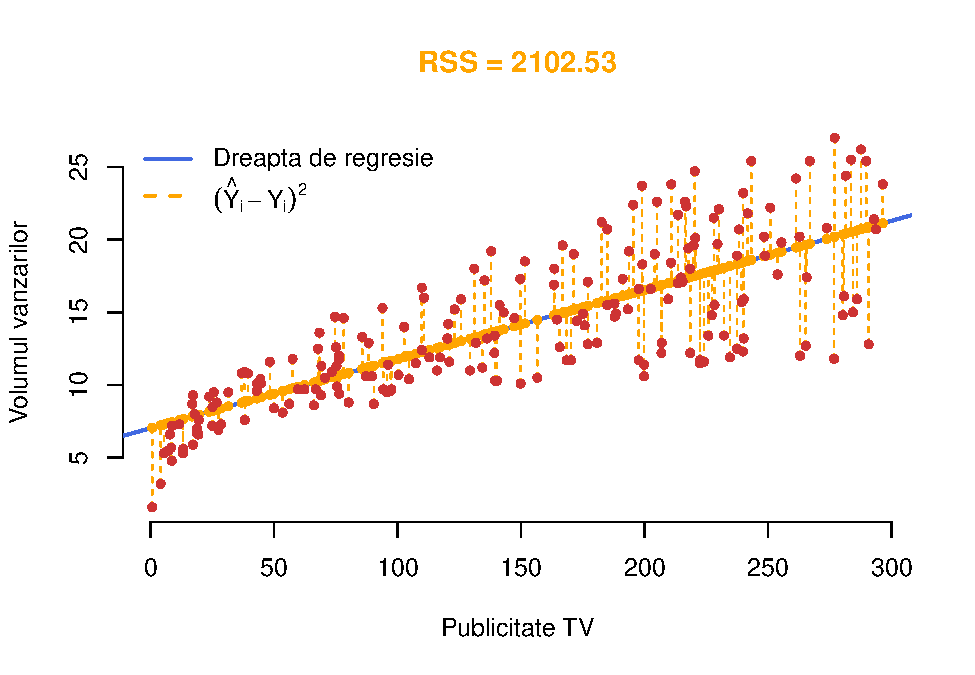
\includegraphics[width=0.8\linewidth]{Lab_5_files/figure-latex/unnamed-chunk-22-1} \end{center}

Tabelul ANOVA se obține prin

\begin{Shaded}
\begin{Highlighting}[]
\CommentTok{# tabel ANOVA }
\KeywordTok{anova}\NormalTok{(advertise_TV_model)}
\NormalTok{Analysis of Variance Table}

\NormalTok{Response}\OperatorTok{:}\StringTok{ }\NormalTok{sales}
\NormalTok{           Df Sum Sq Mean Sq F value    }\KeywordTok{Pr}\NormalTok{(}\OperatorTok{>}\NormalTok{F)    }
\NormalTok{TV          }\DecValTok{1} \FloatTok{3314.6}  \FloatTok{3314.6}  \FloatTok{312.14} \OperatorTok{<}\StringTok{ }\FloatTok{2.2e-16} \OperatorTok{**}\ErrorTok{*}
\NormalTok{Residuals }\DecValTok{198} \FloatTok{2102.5}    \FloatTok{10.6}                      
\OperatorTok{---}
\NormalTok{Signif. codes}\OperatorTok{:}\StringTok{  }\DecValTok{0} \StringTok{'***'} \FloatTok{0.001} \StringTok{'**'} \FloatTok{0.01} \StringTok{'*'} \FloatTok{0.05} \StringTok{'.'} \FloatTok{0.1} \StringTok{' '} \DecValTok{1}
\end{Highlighting}
\end{Shaded}

Definiția \emph{coeficientului de determinare} \(R^2\) este strâns
legată de descompunerea ANOVA:

\[
R^2 = \frac{SS_{reg}}{SS_T}=\frac{SS_T-RSS}{SS_T} = 1 - \frac{RSS}{SS_T}
\]

\(R^2\) măsoară \textbf{proporția din variația} variabilei răspuns \(Y\)
\textbf{explicată} de variabila predictor \(X\) prin regresie. Proporția
din variația totală a lui \(Y\) care nu este explicată este
\(1-R^2 = \frac{RSS}{SS_T}\). Intuitiv, \(R^2\) măsoară cât de bine
modelul de regresie este în concordanță cu datele (cât de strâns este
norul de puncte în jurul dreptei de regresie). Observăm că dacă datele
concordă \emph{perfect} cu modelul (adică \(RSS=0\)) atunci \(R^2=1\).

În cazul problemei noastre avem \$R\^{}2 =\$0.612 prin urmare
aproximativ 61.19\% din variabilitatea volumului vânzărilor este
explicată de bugetul alocat publicității TV.

Putem vedea că \(R^2=r_{xy}^2\), unde \(r_{xy}\) este \emph{coeficientul
de corelație} empiric:

\[
r_{xy}=\frac{S_{xy}}{\sqrt{S_{xx}S_{yy}}}=\frac{\sum_{i=1}^n \left(X_i-\bar X \right)\left(Y_i-\bar Y \right)}{\sqrt{\sum_{i=1}^n \left(X_i-\bar X \right)^2}\sqrt{\sum_{i=1}^n \left(Y_i-\bar Y \right)^2}}
\]

\begin{Shaded}
\begin{Highlighting}[]
\KeywordTok{cor}\NormalTok{(advertise}\OperatorTok{$}\NormalTok{TV, advertise}\OperatorTok{$}\NormalTok{sales)}\OperatorTok{^}\DecValTok{2}
\NormalTok{[}\DecValTok{1}\NormalTok{] }\FloatTok{0.6118751}
\end{Highlighting}
\end{Shaded}

Mai mult se poate verifica și că \(R^2=r^2_{y\hat y}\), adică
\emph{coeficientul de determinare este egal cu pătratul coeficientului
de corelație empirică dintre \(Y_1,\ldots,Y_n\) și
\(\hat Y_1,\ldots,\hat Y_n\)}.

Verificăm relația \(R^2=r^2_{xy}=r^2_{y\hat y}\) numeric:

\begin{Shaded}
\begin{Highlighting}[]
\NormalTok{yHat =}\StringTok{ }\NormalTok{advertise_TV_model}\OperatorTok{$}\NormalTok{fitted.values}

\NormalTok{advertise_TV_model_summary}\OperatorTok{$}\NormalTok{r.squared }\CommentTok{# R^2}
\NormalTok{[}\DecValTok{1}\NormalTok{] }\FloatTok{0.6118751}
\KeywordTok{cor}\NormalTok{(advertise}\OperatorTok{$}\NormalTok{TV, advertise}\OperatorTok{$}\NormalTok{sales)}\OperatorTok{^}\DecValTok{2} \CommentTok{# corelatia^2 dintre x si y}
\NormalTok{[}\DecValTok{1}\NormalTok{] }\FloatTok{0.6118751}
\KeywordTok{cor}\NormalTok{(advertise}\OperatorTok{$}\NormalTok{sales, yHat)}\OperatorTok{^}\DecValTok{2} \CommentTok{# corelatia^2 dintre y si yHat}
\NormalTok{[}\DecValTok{1}\NormalTok{] }\FloatTok{0.6118751}
\end{Highlighting}
\end{Shaded}

\subsection{Inferență asupra
parametrilor}\label{inferenta-asupra-parametrilor}

Este predictorul \(X\) folositor în prezicerea răspunsului \(Y\) ? Vrem
să testăm ipoteza nulă \(H_0:\;\beta_j=0\) (pentru \(j=1\) spunem că
predictorul \texttt{nivel\ de\ sare} nu are un efect \emph{liniar}
semnificativ asupra \texttt{tensiunii\ arteriale}). Pentru aceasta vom
folosi statistica de test

\[
t_j = \frac{\hat{\beta}_j}{\hat{SE}(\hat{\beta_j})}\sim_{H_0} t_{n-2}.
\]

Funcția \texttt{summary} ne întoarce \(p\)-valoarea corespunzătoare a
acestor teste:

\begin{Shaded}
\begin{Highlighting}[]
\KeywordTok{summary}\NormalTok{(advertise_TV_model)}

\NormalTok{Call}\OperatorTok{:}
\KeywordTok{lm}\NormalTok{(}\DataTypeTok{formula =}\NormalTok{ sales }\OperatorTok{~}\StringTok{ }\NormalTok{TV, }\DataTypeTok{data =}\NormalTok{ advertise)}

\NormalTok{Residuals}\OperatorTok{:}
\StringTok{    }\NormalTok{Min      1Q  Median      3Q     Max }
\OperatorTok{-}\FloatTok{8.3860} \OperatorTok{-}\FloatTok{1.9545} \OperatorTok{-}\FloatTok{0.1913}  \FloatTok{2.0671}  \FloatTok{7.2124} 

\NormalTok{Coefficients}\OperatorTok{:}
\StringTok{            }\NormalTok{Estimate Std. Error t value }\KeywordTok{Pr}\NormalTok{(}\OperatorTok{>}\ErrorTok{|}\NormalTok{t}\OperatorTok{|}\NormalTok{)    }
\NormalTok{(Intercept) }\FloatTok{7.032594}   \FloatTok{0.457843}   \FloatTok{15.36}   \OperatorTok{<}\FloatTok{2e-16} \OperatorTok{**}\ErrorTok{*}
\NormalTok{TV          }\FloatTok{0.047537}   \FloatTok{0.002691}   \FloatTok{17.67}   \OperatorTok{<}\FloatTok{2e-16} \OperatorTok{**}\ErrorTok{*}
\OperatorTok{---}
\NormalTok{Signif. codes}\OperatorTok{:}\StringTok{  }\DecValTok{0} \StringTok{'***'} \FloatTok{0.001} \StringTok{'**'} \FloatTok{0.01} \StringTok{'*'} \FloatTok{0.05} \StringTok{'.'} \FloatTok{0.1} \StringTok{' '} \DecValTok{1}

\NormalTok{Residual standard error}\OperatorTok{:}\StringTok{ }\FloatTok{3.259}\NormalTok{ on }\DecValTok{198}\NormalTok{ degrees of freedom}
\NormalTok{Multiple R}\OperatorTok{-}\NormalTok{squared}\OperatorTok{:}\StringTok{  }\FloatTok{0.6119}\NormalTok{,    Adjusted R}\OperatorTok{-}\NormalTok{squared}\OperatorTok{:}\StringTok{  }\FloatTok{0.6099} 
\NormalTok{F}\OperatorTok{-}\NormalTok{statistic}\OperatorTok{:}\StringTok{ }\FloatTok{312.1}\NormalTok{ on }\DecValTok{1}\NormalTok{ and }\DecValTok{198}\NormalTok{ DF,  p}\OperatorTok{-}\NormalTok{value}\OperatorTok{:}\StringTok{ }\ErrorTok{<}\StringTok{ }\FloatTok{2.2e-16}
\end{Highlighting}
\end{Shaded}

Observăm că ambele ipoteze sunt respinse în favoarea alternativelor
bilaterale (la aceeași concluzie am ajuns și utitându-ne la intervalele
de încredere - nu conțineau valoarea \(0\)). Putem observa că \(t_1^2\)
este exact valoarea \(F\) statisticii, deci cele două abordări ne dau
aceleași rezultate numerice.

\subsubsection{Predicție}\label{predictie}

Pentru un nou set de predictori, \(x_0\), răspunsul prognozat este
\(\hat{y} = \hat{\beta}_0+\hat{\beta}_1 x_0\) și vrem să investigăm
incertitudinea din această predicție. Putem face distincția între două
tipuri de predicție: predicție asupra răspunsului viitor mediu
(inferență asupra mediei condiționate \(\mathbb{E}[Y|X=x_0]\)) sau
predicție asupra observațiilor viitoare (inferență asupra răspunsului
condiționat \(Y|X=x_0\)).

Un interval de încredere pentru răspunsul viitor mediu este:

\[
\left(\hat y \pm t_{n-2;1-\alpha/2}\sqrt{\hat\sigma^2\left(\frac{1}{n}+\frac{(x_0-\bar x)^2}{S_{xx}}\right)}\right)
\]

Un interval de încredere pentru valoarea prezisă (interval de predicție)
este:

\[
\left(\hat y \pm t_{n-2;1-\alpha/2}\sqrt{\hat\sigma^2\left(1+\frac{1}{n}+\frac{(x_0-\bar x)^2}{S_{xx}}\right)}\right)
\]

Pentru a găsi aceste intervale vom folosi funcția \texttt{predict()}:

\begin{Shaded}
\begin{Highlighting}[]
\NormalTok{newData =}\StringTok{ }\KeywordTok{data.frame}\NormalTok{(}\DataTypeTok{TV =} \DecValTok{150}\NormalTok{)}
\NormalTok{newData2 =}\StringTok{ }\KeywordTok{data.frame}\NormalTok{(}\DataTypeTok{TV =} \KeywordTok{c}\NormalTok{(}\DecValTok{130}\NormalTok{, }\DecValTok{140}\NormalTok{, }\DecValTok{150}\NormalTok{))}

\CommentTok{# Predictie}
\KeywordTok{predict}\NormalTok{(advertise_TV_model, }\DataTypeTok{newdata =}\NormalTok{ newData)}
       \DecValTok{1} 
\FloatTok{14.16309} 

\CommentTok{# Predictie pentru valoarea raspunsului mediu}
\KeywordTok{predict}\NormalTok{(advertise_TV_model, }\DataTypeTok{newdata =}\NormalTok{ newData, }\DataTypeTok{interval =} \StringTok{"confidence"}\NormalTok{)}
\NormalTok{       fit      lwr      upr}
\DecValTok{1} \FloatTok{14.16309} \FloatTok{13.70842} \FloatTok{14.61776}
\KeywordTok{predict}\NormalTok{(advertise_TV_model, }\DataTypeTok{newdata =}\NormalTok{ newData2, }\DataTypeTok{interval =} \StringTok{"confidence"}\NormalTok{)}
\NormalTok{       fit      lwr      upr}
\DecValTok{1} \FloatTok{13.21236} \FloatTok{12.74905} \FloatTok{13.67566}
\DecValTok{2} \FloatTok{13.68772} \FloatTok{13.23179} \FloatTok{14.14365}
\DecValTok{3} \FloatTok{14.16309} \FloatTok{13.70842} \FloatTok{14.61776}

\CommentTok{# Predictie asupra observatiilor viitoare}
\KeywordTok{predict}\NormalTok{(advertise_TV_model, }\DataTypeTok{newdata =}\NormalTok{ newData, }\DataTypeTok{interval =} \StringTok{"prediction"}\NormalTok{)}
\NormalTok{       fit      lwr      upr}
\DecValTok{1} \FloatTok{14.16309} \FloatTok{7.720898} \FloatTok{20.60528}
\KeywordTok{predict}\NormalTok{(advertise_TV_model, }\DataTypeTok{newdata =}\NormalTok{ newData2, }\DataTypeTok{interval =} \StringTok{"prediction"}\NormalTok{)}
\NormalTok{       fit      lwr      upr}
\DecValTok{1} \FloatTok{13.21236} \FloatTok{6.769550} \FloatTok{19.65516}
\DecValTok{2} \FloatTok{13.68772} \FloatTok{7.245442} \FloatTok{20.13000}
\DecValTok{3} \FloatTok{14.16309} \FloatTok{7.720898} \FloatTok{20.60528}
\end{Highlighting}
\end{Shaded}

Volumul de vânzări prezis pentru o anumită valoare \(x_0\) impreună cu
intervalul de încredere de nivel 95\% pentru răspunsul mediu și cu
intervalul de predicție, sunt ilustrate în figura următoare

\begin{Shaded}
\begin{Highlighting}[]
\NormalTok{alpha =}\StringTok{ }\FloatTok{0.05}
\NormalTok{x0 =}\StringTok{ }\KeywordTok{c}\NormalTok{(}\DecValTok{155}\NormalTok{, }\DecValTok{294}\NormalTok{)}

\NormalTok{p.conf =}\StringTok{ }\KeywordTok{predict}\NormalTok{(advertise_TV_model, }\KeywordTok{data.frame}\NormalTok{(}\DataTypeTok{TV =}\NormalTok{ x0), }\DataTypeTok{se =}\NormalTok{ T, }\DataTypeTok{interval =} \StringTok{"confidence"}\NormalTok{)}
\NormalTok{p.pred =}\StringTok{ }\KeywordTok{predict}\NormalTok{(advertise_TV_model, }\KeywordTok{data.frame}\NormalTok{(}\DataTypeTok{TV =}\NormalTok{ x0), }\DataTypeTok{se =}\NormalTok{ T, }\DataTypeTok{interval =} \StringTok{"prediction"}\NormalTok{)}

\CommentTok{# diagrama de imprastiesre}
\KeywordTok{plot}\NormalTok{(advertise}\OperatorTok{$}\NormalTok{TV, advertise}\OperatorTok{$}\NormalTok{sales,}
     \DataTypeTok{col =} \StringTok{"grey70"}\NormalTok{, }\DataTypeTok{pch =} \DecValTok{20}\NormalTok{,}
     \DataTypeTok{xlab =} \StringTok{"Publicitate TV"}\NormalTok{,}
     \DataTypeTok{ylab =} \StringTok{"Volumul vanzarilor"}\NormalTok{,}
     \DataTypeTok{bty =} \StringTok{"n"}\NormalTok{)}

\CommentTok{# dreapta de regresie}
\KeywordTok{abline}\NormalTok{(advertise_TV_model}\OperatorTok{$}\NormalTok{coefficients, }\DataTypeTok{col =} \StringTok{"royalblue"}\NormalTok{, }\DataTypeTok{lwd =} \DecValTok{2}\NormalTok{)}

\CommentTok{#intervalele de incredere}
\KeywordTok{segments}\NormalTok{(}\DataTypeTok{x0 =}\NormalTok{ x0, }\DataTypeTok{y0 =}\NormalTok{ p.conf}\OperatorTok{$}\NormalTok{fit[,}\DecValTok{2}\NormalTok{], }\DataTypeTok{x1 =}\NormalTok{ x0, }\DataTypeTok{y1 =}\NormalTok{ p.conf}\OperatorTok{$}\NormalTok{fit[,}\DecValTok{3}\NormalTok{], }
         \DataTypeTok{col =} \StringTok{"orange"}\NormalTok{, }\DataTypeTok{lty =} \DecValTok{1}\NormalTok{, }\DataTypeTok{lwd =} \DecValTok{2}\NormalTok{)}
\KeywordTok{segments}\NormalTok{(}\DataTypeTok{x0 =}\NormalTok{ x0}\OperatorTok{-}\FloatTok{2.5}\NormalTok{, }\DataTypeTok{y0 =}\NormalTok{ p.conf}\OperatorTok{$}\NormalTok{fit[,}\DecValTok{2}\NormalTok{], }\DataTypeTok{x1 =}\NormalTok{ x0}\OperatorTok{+}\FloatTok{2.5}\NormalTok{, }\DataTypeTok{y1 =}\NormalTok{ p.conf}\OperatorTok{$}\NormalTok{fit[,}\DecValTok{2}\NormalTok{], }
         \DataTypeTok{col =} \StringTok{"orange"}\NormalTok{, }\DataTypeTok{lty =} \DecValTok{1}\NormalTok{, }\DataTypeTok{lwd =} \DecValTok{2}\NormalTok{)}
\KeywordTok{segments}\NormalTok{(}\DataTypeTok{x0 =}\NormalTok{ x0}\OperatorTok{-}\FloatTok{2.5}\NormalTok{, }\DataTypeTok{y0 =}\NormalTok{ p.conf}\OperatorTok{$}\NormalTok{fit[,}\DecValTok{3}\NormalTok{], }\DataTypeTok{x1 =}\NormalTok{ x0}\OperatorTok{+}\FloatTok{2.5}\NormalTok{, }\DataTypeTok{y1 =}\NormalTok{ p.conf}\OperatorTok{$}\NormalTok{fit[,}\DecValTok{3}\NormalTok{], }
         \DataTypeTok{col =} \StringTok{"orange"}\NormalTok{, }\DataTypeTok{lty =} \DecValTok{1}\NormalTok{, }\DataTypeTok{lwd =} \DecValTok{2}\NormalTok{)}

\CommentTok{#intervalele de predictie}
\KeywordTok{segments}\NormalTok{(}\DataTypeTok{x0 =}\NormalTok{ x0, }\DataTypeTok{y0 =}\NormalTok{ p.pred}\OperatorTok{$}\NormalTok{fit[,}\DecValTok{2}\NormalTok{], }\DataTypeTok{x1 =}\NormalTok{ x0, }\DataTypeTok{y1 =}\NormalTok{ p.pred}\OperatorTok{$}\NormalTok{fit[,}\DecValTok{3}\NormalTok{], }
         \DataTypeTok{col =} \StringTok{"magenta"}\NormalTok{, }\DataTypeTok{lty =} \DecValTok{2}\NormalTok{, }\DataTypeTok{lwd =} \DecValTok{2}\NormalTok{)}
\KeywordTok{segments}\NormalTok{(}\DataTypeTok{x0 =}\NormalTok{ x0}\OperatorTok{-}\FloatTok{2.5}\NormalTok{, }\DataTypeTok{y0 =}\NormalTok{ p.pred}\OperatorTok{$}\NormalTok{fit[,}\DecValTok{2}\NormalTok{], }\DataTypeTok{x1 =}\NormalTok{ x0}\OperatorTok{+}\FloatTok{2.5}\NormalTok{, }\DataTypeTok{y1 =}\NormalTok{ p.pred}\OperatorTok{$}\NormalTok{fit[,}\DecValTok{2}\NormalTok{], }
         \DataTypeTok{col =} \StringTok{"magenta"}\NormalTok{, }\DataTypeTok{lty =} \DecValTok{2}\NormalTok{, }\DataTypeTok{lwd =} \DecValTok{2}\NormalTok{)}
\KeywordTok{segments}\NormalTok{(}\DataTypeTok{x0 =}\NormalTok{ x0}\OperatorTok{-}\FloatTok{2.5}\NormalTok{, }\DataTypeTok{y0 =}\NormalTok{ p.pred}\OperatorTok{$}\NormalTok{fit[,}\DecValTok{3}\NormalTok{], }\DataTypeTok{x1 =}\NormalTok{ x0}\OperatorTok{+}\FloatTok{2.5}\NormalTok{, }\DataTypeTok{y1 =}\NormalTok{ p.pred}\OperatorTok{$}\NormalTok{fit[,}\DecValTok{3}\NormalTok{], }
         \DataTypeTok{col =} \StringTok{"magenta"}\NormalTok{, }\DataTypeTok{lty =} \DecValTok{2}\NormalTok{, }\DataTypeTok{lwd =} \DecValTok{2}\NormalTok{)}

\CommentTok{# valoarea prezisa}
\KeywordTok{points}\NormalTok{(x0, p.conf}\OperatorTok{$}\NormalTok{fit[,}\DecValTok{1}\NormalTok{], }
       \DataTypeTok{col =} \StringTok{"brown3"}\NormalTok{, }
       \DataTypeTok{pch =} \DecValTok{20}\NormalTok{)}

\KeywordTok{legend}\NormalTok{(}\StringTok{"topleft"}\NormalTok{, }
       \DataTypeTok{legend =} \KeywordTok{c}\NormalTok{(}\StringTok{"Dreapta de regresie"}\NormalTok{, }
                  \StringTok{"interval de incredere"}\NormalTok{,}
                  \StringTok{"interval de predictie"}\NormalTok{), }
       \DataTypeTok{lwd =} \KeywordTok{c}\NormalTok{(}\DecValTok{2}\NormalTok{, }\DecValTok{2}\NormalTok{, }\DecValTok{2}\NormalTok{),}
       \DataTypeTok{col =} \KeywordTok{c}\NormalTok{(}\StringTok{"royalblue"}\NormalTok{, }\StringTok{"orange"}\NormalTok{, }\StringTok{"magenta"}\NormalTok{), }
       \DataTypeTok{lty =} \KeywordTok{c}\NormalTok{(}\DecValTok{1}\NormalTok{, }\DecValTok{2}\NormalTok{, }\DecValTok{2}\NormalTok{), }
       \DataTypeTok{bty =} \StringTok{"n"}\NormalTok{)}
\end{Highlighting}
\end{Shaded}

\begin{center}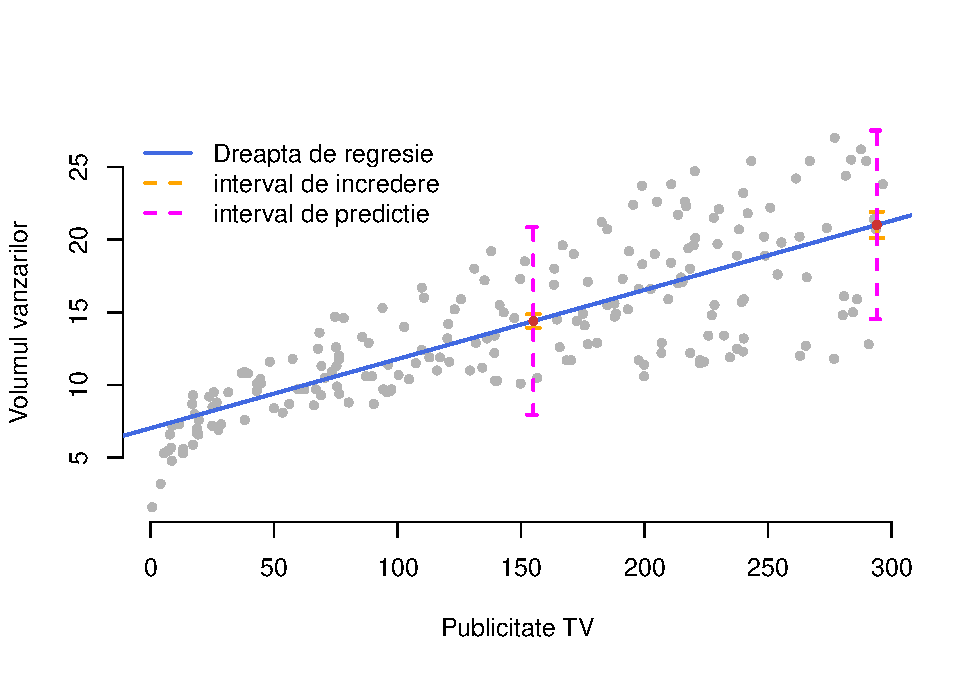
\includegraphics[width=0.8\linewidth]{Lab_5_files/figure-latex/unnamed-chunk-28-1} \end{center}

Sunt circumstanțe în care am dori să avem intervalele de încredere
pentru răspunsul mediu în mai mult de un punct, prin urmare ne aflăm în
cadrul unei probleme de inferență simultană. O soluție la această
problemă, în cazul în care avem \(m\) puncte, este dată de inegalitatea
lui Bonferroni care conduce la marginea

\[
  \hat \beta_0 + \hat\beta_1 x_{0i} - t_{n-2, \frac{\alpha}{2m}}RSS\sqrt{\frac{1}{n}+\frac{(x_{0i} - \bar{x})^2}{S_{xx}}} < \beta_0 + \beta_1 x_{0i} < \hat \beta_0 + \hat\beta_1 x_{0i} + t_{n-2, \frac{\alpha}{2m}}RSS\sqrt{\frac{1}{n}+\frac{(x_{0i} - \bar{x})^2}{S_{xx}}}.
\]

Scheffe (a se vedea \citep[pag. 559 - 562]{Casella2001}) a arătat,
pentru problema de regresie, că există un interval care este adevărat
pentru orice \(x\)

\[
  \hat \beta_0 + \hat\beta_1 x - M_{\alpha}RSS\sqrt{\frac{1}{n}+\frac{(x - \bar{x})^2}{S_{xx}}} < \beta_0 + \beta_1 x < \hat \beta_0 + \hat\beta_1 x + M_{\alpha}RSS\sqrt{\frac{1}{n}+\frac{(x - \bar{x})^2}{S_{xx}}}, \forall x
\]

unde \(M_{\alpha} = \sqrt{2f_{2, n-2}^{\alpha}}\).

În figura de mai jos am ilustrat volumul de vânzări prezis împreună cu
intervalul de încredere de nivel 95\% pentru răspunsul mediu folosind 6
intervale de tip Bonferroni precum și banda lui Scheffe:

\begin{Shaded}
\begin{Highlighting}[]
\NormalTok{alpha =}\StringTok{ }\FloatTok{0.05}
\NormalTok{g =}\StringTok{ }\KeywordTok{seq}\NormalTok{(}\DecValTok{5}\NormalTok{,}\DecValTok{300}\NormalTok{,}\FloatTok{0.5}\NormalTok{)}

\NormalTok{p =}\StringTok{ }\KeywordTok{predict}\NormalTok{(advertise_TV_model, }\KeywordTok{data.frame}\NormalTok{(}\DataTypeTok{TV =}\NormalTok{ g), }\DataTypeTok{se =}\NormalTok{ T, }\DataTypeTok{interval =} \StringTok{"confidence"}\NormalTok{)}

\KeywordTok{matplot}\NormalTok{(g, p}\OperatorTok{$}\NormalTok{fit, }\DataTypeTok{type =} \StringTok{"l"}\NormalTok{, }\DataTypeTok{lty =} \KeywordTok{c}\NormalTok{(}\DecValTok{1}\NormalTok{,}\DecValTok{2}\NormalTok{,}\DecValTok{2}\NormalTok{), }
        \DataTypeTok{lwd =} \KeywordTok{c}\NormalTok{(}\DecValTok{2}\NormalTok{,}\DecValTok{1}\NormalTok{,}\DecValTok{1}\NormalTok{),}
        \DataTypeTok{col =} \KeywordTok{c}\NormalTok{(}\StringTok{"royalblue"}\NormalTok{, }\StringTok{"grey50"}\NormalTok{, }\StringTok{"grey50"}\NormalTok{),}
        \DataTypeTok{xlab =} \StringTok{"Publicitate TV"}\NormalTok{,}
        \DataTypeTok{ylab =} \StringTok{"Volumul vanzarilor"}\NormalTok{,}
        \DataTypeTok{bty =} \StringTok{"n"}\NormalTok{)}

\CommentTok{# rug(advertise$TV)}

\KeywordTok{points}\NormalTok{(advertise}\OperatorTok{$}\NormalTok{TV, advertise}\OperatorTok{$}\NormalTok{sales, }
       \DataTypeTok{col =} \StringTok{"grey70"}\NormalTok{, }\DataTypeTok{pch =} \DecValTok{20}\NormalTok{)}
\KeywordTok{abline}\NormalTok{(}\DataTypeTok{v =} \KeywordTok{mean}\NormalTok{(advertise}\OperatorTok{$}\NormalTok{TV), }\DataTypeTok{lty =} \DecValTok{3}\NormalTok{, }\DataTypeTok{col =} \StringTok{"grey65"}\NormalTok{)}

\CommentTok{# Scheffe's bounds}
\NormalTok{M =}\StringTok{ }\KeywordTok{sqrt}\NormalTok{(}\DecValTok{2}\OperatorTok{*}\KeywordTok{qf}\NormalTok{(}\DecValTok{1}\OperatorTok{-}\NormalTok{alpha, }\DecValTok{2}\NormalTok{, n}\OperatorTok{-}\DecValTok{2}\NormalTok{))}

\NormalTok{s_xx =}\StringTok{ }\NormalTok{(n}\OperatorTok{-}\DecValTok{1}\NormalTok{)}\OperatorTok{*}\KeywordTok{var}\NormalTok{(advertise}\OperatorTok{$}\NormalTok{TV)}
\NormalTok{lw_scheffe =}\StringTok{ }\NormalTok{b0 }\OperatorTok{+}\StringTok{ }\NormalTok{b1}\OperatorTok{*}\NormalTok{g }\OperatorTok{-}\StringTok{ }\NormalTok{M}\OperatorTok{*}\NormalTok{sigma_hat}\OperatorTok{*}\KeywordTok{sqrt}\NormalTok{(}\DecValTok{1}\OperatorTok{/}\NormalTok{n}\OperatorTok{+}\NormalTok{(g}\OperatorTok{-}\KeywordTok{mean}\NormalTok{(advertise}\OperatorTok{$}\NormalTok{TV))}\OperatorTok{^}\DecValTok{2}\OperatorTok{/}\NormalTok{s_xx)}
\NormalTok{up_scheffe =}\StringTok{ }\NormalTok{b0 }\OperatorTok{+}\StringTok{ }\NormalTok{b1}\OperatorTok{*}\NormalTok{g }\OperatorTok{+}\StringTok{ }\NormalTok{M}\OperatorTok{*}\NormalTok{sigma_hat}\OperatorTok{*}\KeywordTok{sqrt}\NormalTok{(}\DecValTok{1}\OperatorTok{/}\NormalTok{n}\OperatorTok{+}\NormalTok{(g}\OperatorTok{-}\KeywordTok{mean}\NormalTok{(advertise}\OperatorTok{$}\NormalTok{TV))}\OperatorTok{^}\DecValTok{2}\OperatorTok{/}\NormalTok{s_xx)}

\KeywordTok{lines}\NormalTok{(g, lw_scheffe, }
      \DataTypeTok{lty =} \DecValTok{4}\NormalTok{, }
      \DataTypeTok{lwd =} \DecValTok{2}\NormalTok{,}
      \DataTypeTok{col =} \StringTok{"brown4"}\NormalTok{)}
\KeywordTok{lines}\NormalTok{(g, up_scheffe, }
      \DataTypeTok{lty =} \DecValTok{4}\NormalTok{, }
      \DataTypeTok{lwd =} \DecValTok{2}\NormalTok{,}
      \DataTypeTok{col =} \StringTok{"brown4"}\NormalTok{)}

\CommentTok{# Bonferroni bounds}

\NormalTok{x0 =}\StringTok{ }\KeywordTok{runif}\NormalTok{(}\DecValTok{6}\NormalTok{, }\DataTypeTok{min =} \DecValTok{10}\NormalTok{, }\DataTypeTok{max =} \DecValTok{290}\NormalTok{)}
\NormalTok{m =}\StringTok{ }\KeywordTok{length}\NormalTok{(x0)}

\NormalTok{t_bonf =}\StringTok{ }\KeywordTok{qt}\NormalTok{(}\DecValTok{1}\OperatorTok{-}\NormalTok{alpha}\OperatorTok{/}\NormalTok{(}\DecValTok{2}\OperatorTok{*}\NormalTok{m), n}\OperatorTok{-}\DecValTok{2}\NormalTok{)}

\NormalTok{lw_bonf =}\StringTok{ }\NormalTok{b0 }\OperatorTok{+}\StringTok{ }\NormalTok{b1}\OperatorTok{*}\NormalTok{x0 }\OperatorTok{-}\StringTok{ }\NormalTok{t_bonf}\OperatorTok{*}\NormalTok{sigma_hat}\OperatorTok{*}\KeywordTok{sqrt}\NormalTok{(}\DecValTok{1}\OperatorTok{/}\NormalTok{n}\OperatorTok{+}\NormalTok{(x0}\OperatorTok{-}\KeywordTok{mean}\NormalTok{(advertise}\OperatorTok{$}\NormalTok{TV))}\OperatorTok{^}\DecValTok{2}\OperatorTok{/}\NormalTok{s_xx)}
\NormalTok{up_bonf =}\StringTok{ }\NormalTok{b0 }\OperatorTok{+}\StringTok{ }\NormalTok{b1}\OperatorTok{*}\NormalTok{x0 }\OperatorTok{+}\StringTok{ }\NormalTok{t_bonf}\OperatorTok{*}\NormalTok{sigma_hat}\OperatorTok{*}\KeywordTok{sqrt}\NormalTok{(}\DecValTok{1}\OperatorTok{/}\NormalTok{n}\OperatorTok{+}\NormalTok{(x0}\OperatorTok{-}\KeywordTok{mean}\NormalTok{(advertise}\OperatorTok{$}\NormalTok{TV))}\OperatorTok{^}\DecValTok{2}\OperatorTok{/}\NormalTok{s_xx)}

\KeywordTok{segments}\NormalTok{(}\DataTypeTok{x0 =}\NormalTok{ x0, }\DataTypeTok{y0 =}\NormalTok{ lw_bonf, }\DataTypeTok{x1 =}\NormalTok{ x0, }\DataTypeTok{y1 =}\NormalTok{ up_bonf, }
         \DataTypeTok{col =} \StringTok{"orange"}\NormalTok{, }\DataTypeTok{lty =} \DecValTok{1}\NormalTok{, }\DataTypeTok{lwd =} \DecValTok{2}\NormalTok{)}
\KeywordTok{segments}\NormalTok{(}\DataTypeTok{x0 =}\NormalTok{ x0}\OperatorTok{-}\FloatTok{1.25}\NormalTok{, }\DataTypeTok{y0 =}\NormalTok{ lw_bonf, }\DataTypeTok{x1 =}\NormalTok{ x0}\OperatorTok{+}\FloatTok{1.25}\NormalTok{, }\DataTypeTok{y1 =}\NormalTok{ lw_bonf, }
         \DataTypeTok{col =} \StringTok{"orange"}\NormalTok{, }\DataTypeTok{lty =} \DecValTok{1}\NormalTok{, }\DataTypeTok{lwd =} \DecValTok{2}\NormalTok{)}
\KeywordTok{segments}\NormalTok{(}\DataTypeTok{x0 =}\NormalTok{ x0}\OperatorTok{-}\FloatTok{1.25}\NormalTok{, }\DataTypeTok{y0 =}\NormalTok{ up_bonf, }\DataTypeTok{x1 =}\NormalTok{ x0}\OperatorTok{+}\FloatTok{1.25}\NormalTok{, }\DataTypeTok{y1 =}\NormalTok{ up_bonf, }
         \DataTypeTok{col =} \StringTok{"orange"}\NormalTok{, }\DataTypeTok{lty =} \DecValTok{1}\NormalTok{, }\DataTypeTok{lwd =} \DecValTok{2}\NormalTok{)}

\KeywordTok{legend}\NormalTok{(}\StringTok{"topleft"}\NormalTok{, }\DataTypeTok{legend =} \KeywordTok{c}\NormalTok{(}\StringTok{"Dreapta de regresie"}\NormalTok{, }\StringTok{"95% t interval"}\NormalTok{, }
                                      \StringTok{"95% Scheffe interval"}\NormalTok{, }
                             \KeywordTok{paste0}\NormalTok{(m, }\StringTok{" intervale Bonferroni (95%)"}\NormalTok{)), }
       \DataTypeTok{lwd =} \KeywordTok{c}\NormalTok{(}\DecValTok{2}\NormalTok{, }\DecValTok{2}\NormalTok{, }\DecValTok{2}\NormalTok{, }\DecValTok{2}\NormalTok{),}
       \DataTypeTok{col =} \KeywordTok{c}\NormalTok{(}\StringTok{"royalblue"}\NormalTok{, }\StringTok{"grey50"}\NormalTok{, }\StringTok{"brown4"}\NormalTok{, }\StringTok{"orange"}\NormalTok{), }
       \DataTypeTok{lty =} \KeywordTok{c}\NormalTok{(}\DecValTok{1}\NormalTok{, }\DecValTok{2}\NormalTok{, }\DecValTok{4}\NormalTok{, }\DecValTok{1}\NormalTok{), }
       \DataTypeTok{bty =} \StringTok{"n"}\NormalTok{)}
\end{Highlighting}
\end{Shaded}

\begin{center}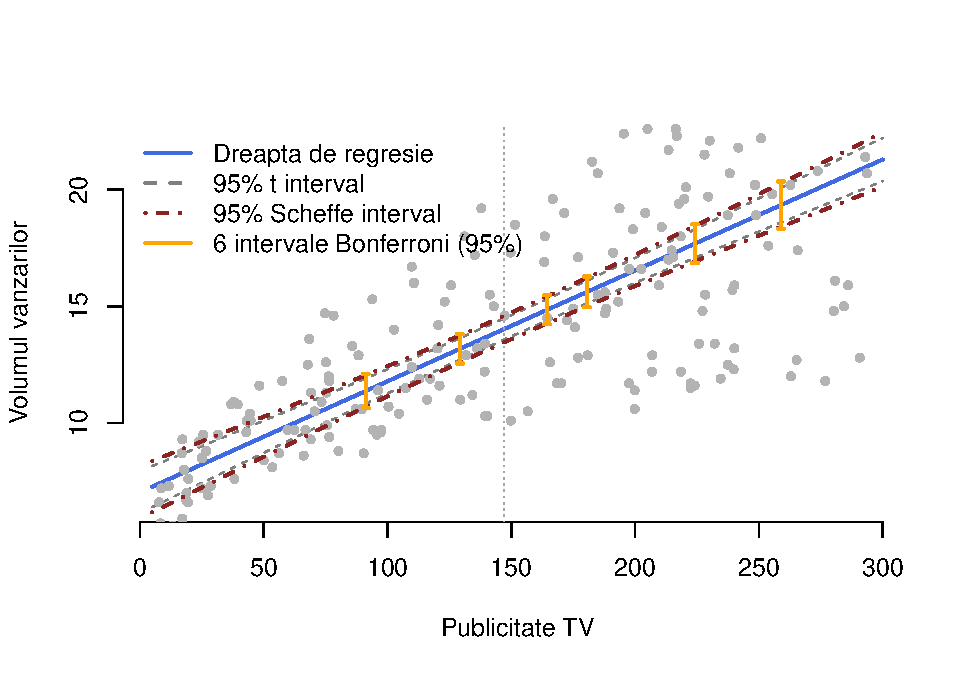
\includegraphics[width=0.8\linewidth]{Lab_5_files/figure-latex/unnamed-chunk-29-1} \end{center}

\subsection{Diagnostic}\label{diagnostic}

În această secțiune vom vedea dacă setul nostru de date verifică
ipotezele modelului de regresie liniară.

\begin{enumerate}
\def\labelenumi{\alph{enumi})}
\tightlist
\item
  \emph{Independența}
\end{enumerate}

Ipoteza de independență a variabilei răspuns (prin urmare și a erorilor)
reiese, de cele mai multe ori, din modalitatea în care s-a desfășurat
experimentul.

\begin{enumerate}
\def\labelenumi{\alph{enumi})}
\setcounter{enumi}{1}
\tightlist
\item
  \emph{Normalitatea}
\end{enumerate}

Pentru a verifica dacă ipoteza de normalitate a erorilor este
satisfăcută vom trasa dreapta lui Henry (sau Q-Q plot-ul):

\begin{Shaded}
\begin{Highlighting}[]
\CommentTok{# library(car)}
\KeywordTok{par}\NormalTok{(}\DataTypeTok{bty =} \StringTok{"n"}\NormalTok{)}
\KeywordTok{qqPlot}\NormalTok{(advertise_TV_model, }\DataTypeTok{col =} \StringTok{"brown3"}\NormalTok{, }\DataTypeTok{col.lines =} \StringTok{"grey50"}\NormalTok{, }\DataTypeTok{pch =} \DecValTok{16}\NormalTok{,}
       \DataTypeTok{simulate =} \OtherTok{TRUE}\NormalTok{,}
       \DataTypeTok{xlab =} \StringTok{"Cuantile teoretice"}\NormalTok{,}
       \DataTypeTok{ylab =} \StringTok{"Reziduuri studentizate"}\NormalTok{, }
       \DataTypeTok{main =} \StringTok{"Q-Q plot (Dreapta lui Henry)"}\NormalTok{,}
       \DataTypeTok{bty =} \StringTok{"n"}\NormalTok{)}
\end{Highlighting}
\end{Shaded}

\begin{center}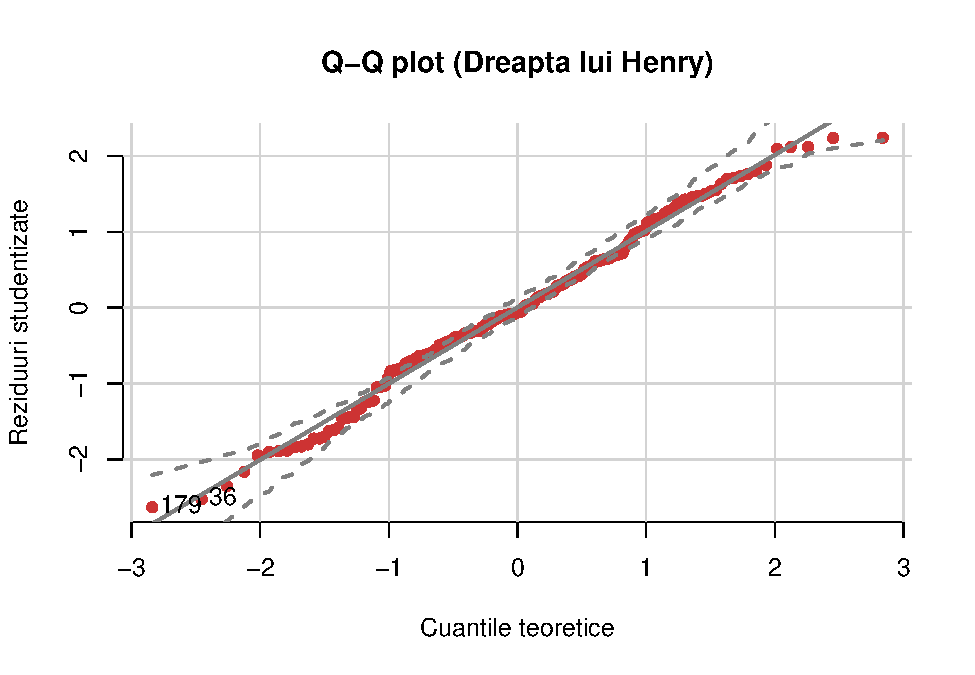
\includegraphics[width=0.8\linewidth]{Lab_5_files/figure-latex/unnamed-chunk-30-1} \end{center}

\begin{verbatim}
[1]  36 179
\end{verbatim}

Putem folosi și testul \texttt{Shapiro-Wilk}:

\begin{Shaded}
\begin{Highlighting}[]
\KeywordTok{shapiro.test}\NormalTok{(}\KeywordTok{residuals}\NormalTok{(advertise_TV_model))}

\NormalTok{    Shapiro}\OperatorTok{-}\NormalTok{Wilk normality test}

\NormalTok{data}\OperatorTok{:}\StringTok{  }\KeywordTok{residuals}\NormalTok{(advertise_TV_model)}
\NormalTok{W =}\StringTok{ }\FloatTok{0.99053}\NormalTok{, p}\OperatorTok{-}\NormalTok{value =}\StringTok{ }\FloatTok{0.2133}
\end{Highlighting}
\end{Shaded}

\begin{enumerate}
\def\labelenumi{\alph{enumi})}
\setcounter{enumi}{2}
\tightlist
\item
  \emph{Homoscedasticitatea}
\end{enumerate}

Pentru a verifica proprietatea de homoscedasticitate a erorilor vom
trasa un grafic al reziduurilor versus valorile prezise (fitted), i.e.
\(\hat{\varepsilon}\) vs \(\hat{y}\). Dacă avem homoscedasticitate a
erorilor atunci ar trebui să vedem o variație constantă pe verticală
(\(\hat{\varepsilon}\)).

Tot în acest grafic putem observa dacă ipoteza de liniaritate este
verificată (în caz de liniaritate între variabila răspuns și variabila
explicativă nu are trebui să vedem o relație sistematică între reziduuri
și valorile prezise - ceea ce nu se întâmplă în cazul nostru) ori dacă
există o altă legătură structurală între variabila dependentă (răspuns)
și cea independentă (predictor).

În cazul aplicației noastre avem următoarea figură:

\begin{Shaded}
\begin{Highlighting}[]
\KeywordTok{plot}\NormalTok{(}\KeywordTok{residuals}\NormalTok{(advertise_TV_model)}\OperatorTok{~}\KeywordTok{fitted}\NormalTok{(advertise_TV_model),  }
     \DataTypeTok{col =} \StringTok{"grey70"}\NormalTok{, }\DataTypeTok{pch =} \DecValTok{16}\NormalTok{, }
     \DataTypeTok{xlab =} \StringTok{"Valori prezise (fitted)"}\NormalTok{,}
     \DataTypeTok{ylab =} \StringTok{"Reziduuri"}\NormalTok{, }
     \DataTypeTok{main =} \StringTok{"Reziduuri vs Valori prezise"}\NormalTok{,}
     \DataTypeTok{bty =} \StringTok{"n"}\NormalTok{)}

\KeywordTok{abline}\NormalTok{(}\DataTypeTok{h =} \DecValTok{0}\NormalTok{, }\DataTypeTok{col =} \StringTok{"grey30"}\NormalTok{)}
\end{Highlighting}
\end{Shaded}

\begin{center}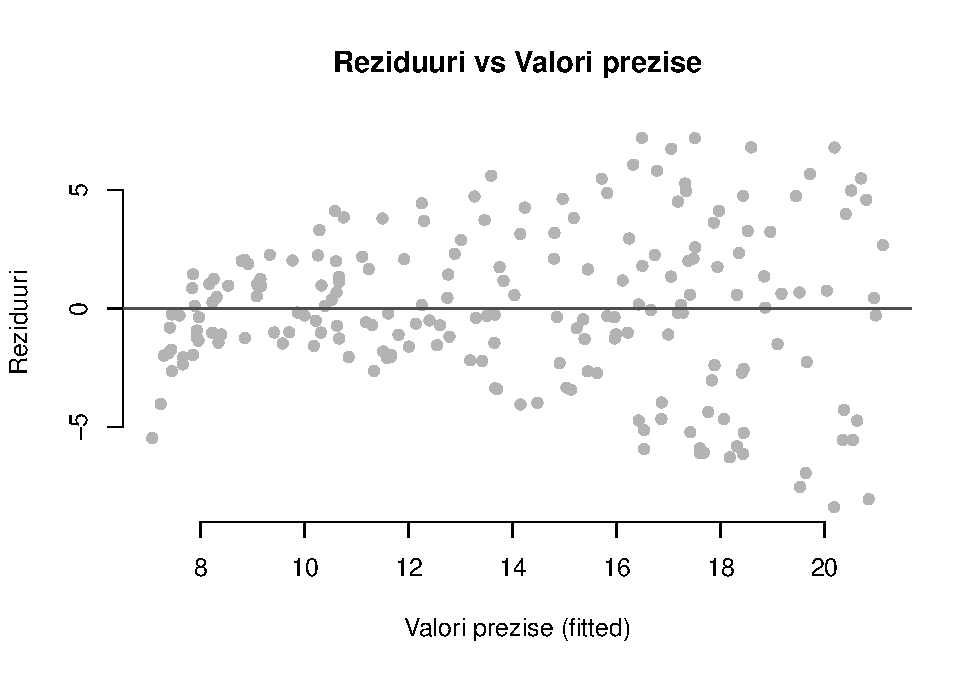
\includegraphics[width=0.8\linewidth]{Lab_5_files/figure-latex/unnamed-chunk-33-1} \end{center}

Se poate observa că magnitudinea valorilor reziduale crește odată cu
magnitudinea valorilor prezise (graficul are o formă de pâlnie) prin
urmare ipoteza de homoscedasticitate nu este satisfăcută. O soluție în
acest caz este de a transforma variabila răspuns \(Y\) cu ajutorul unei
funcții concave, i.e. \(\log{Y}\) sau \(\sqrt{Y}\).

\begin{Shaded}
\begin{Highlighting}[]

\NormalTok{advertise_TV_model_log =}\StringTok{ }\KeywordTok{lm}\NormalTok{(}\KeywordTok{log}\NormalTok{(sales) }\OperatorTok{~}\StringTok{ }\NormalTok{TV, }\DataTypeTok{data =}\NormalTok{ advertise)}
\NormalTok{advertise_TV_model_sqrt =}\StringTok{ }\KeywordTok{lm}\NormalTok{(}\KeywordTok{sqrt}\NormalTok{(sales) }\OperatorTok{~}\StringTok{ }\NormalTok{TV, }\DataTypeTok{data =}\NormalTok{ advertise)}

\KeywordTok{par}\NormalTok{(}\DataTypeTok{mfrow =} \KeywordTok{c}\NormalTok{(}\DecValTok{1}\NormalTok{, }\DecValTok{2}\NormalTok{))}

\KeywordTok{plot}\NormalTok{(}\KeywordTok{residuals}\NormalTok{(advertise_TV_model_log)}\OperatorTok{~}\KeywordTok{fitted}\NormalTok{(advertise_TV_model_log),  }
     \DataTypeTok{col =} \StringTok{"grey70"}\NormalTok{, }\DataTypeTok{pch =} \DecValTok{20}\NormalTok{, }
     \DataTypeTok{xlab =} \StringTok{"Valori prezise (fitted)"}\NormalTok{,}
     \DataTypeTok{ylab =} \StringTok{"Reziduuri"}\NormalTok{, }
     \DataTypeTok{main =} \StringTok{"Reziduuri vs Valori prezise }\CharTok{\textbackslash{}n}\StringTok{(logaritm)"}\NormalTok{,}
     \DataTypeTok{bty =} \StringTok{"n"}\NormalTok{)}

\KeywordTok{abline}\NormalTok{(}\DataTypeTok{h =} \DecValTok{0}\NormalTok{, }\DataTypeTok{col =} \StringTok{"grey30"}\NormalTok{, }\DataTypeTok{lty =} \DecValTok{2}\NormalTok{)}

\KeywordTok{plot}\NormalTok{(}\KeywordTok{residuals}\NormalTok{(advertise_TV_model_sqrt)}\OperatorTok{~}\KeywordTok{fitted}\NormalTok{(advertise_TV_model_sqrt),  }
     \DataTypeTok{col =} \StringTok{"grey70"}\NormalTok{, }\DataTypeTok{pch =} \DecValTok{20}\NormalTok{, }
     \DataTypeTok{xlab =} \StringTok{"Valori prezise (fitted)"}\NormalTok{,}
     \DataTypeTok{ylab =} \StringTok{"Reziduuri"}\NormalTok{, }
     \DataTypeTok{main =} \StringTok{"Reziduuri vs Valori prezise }\CharTok{\textbackslash{}n}\StringTok{(radical)"}\NormalTok{,}
     \DataTypeTok{bty =} \StringTok{"n"}\NormalTok{)}

\KeywordTok{abline}\NormalTok{(}\DataTypeTok{h =} \DecValTok{0}\NormalTok{, }\DataTypeTok{col =} \StringTok{"grey30"}\NormalTok{, }\DataTypeTok{lty =} \DecValTok{2}\NormalTok{)}
\end{Highlighting}
\end{Shaded}

\begin{center}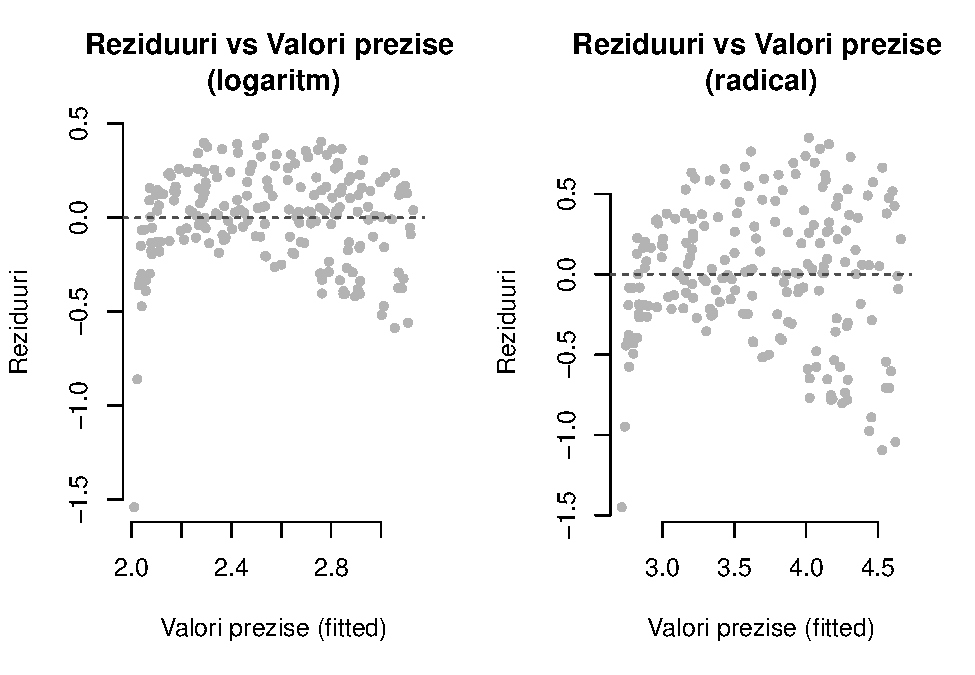
\includegraphics[width=0.8\linewidth]{Lab_5_files/figure-latex/unnamed-chunk-34-1} \end{center}

Observăm că în cazul transformării logaritmice
(\(\log{Y}\approx \beta_0 + \beta_1 x + \varepsilon\)) reziduurile par
să îndeplinească ipoteza de homoscedasticitate (au varianță constantă).
Cu toate acestea, graficul prezintă dovezi ale unei relații neliniare
între volumul vânzărilor și bugetul alocat publicității TV.

\renewcommand\refname{Referințe}
\bibliography{references/InstStatFin2018ref.bib}


\end{document}
